\chapter[Deep neural network applications]{Deep neural network applications on image processing and particle identification} \label{sec:NN_img}
Machine learning algorithms are powerful and versatile tools that can improve the process of data analysis through a learning process from known training datasets of a neural network that is then used for unknown data categorisation. Modern science, including physics, is taking more and more advantage of these techniques as the years go by.
The availability of big data is a key aspect in performing these studies and experimental particle physics is an area inside which properly labelled large datasets can be provided, for training, via test beams and simulations.\\

This chapter describes a possible application of deep neural networks on data generated through the IDEA DR Calorimeter full simulation with the aim to identify particles by analysing the spatial distribution of the deposited energy.\\
An introduction to the computational techniques is provided, briefly describing the role of each component and the common structures that are used in our study.\\

Section \ref{sec:NN_data} describes how data from the IDEA dual-readout calorimeter can be shaped in order to be passed as inputs in image processing neural networks.
%shows which information has been used and how it has been processed to be analyzed by the deep learning algorithms.
After that, the Neural Network (NN) structures are presented in details showing the performance obtained in the training and testing phases, on particle ID tasks.\\
%Eventually the study has been performed extending the energy range, the impact of this generalization conclude the chapter.\\
%\newpage

\section{Physics benchmark}
The chosen task is to recognise and distinguish neutral pions and photons by analysing the spatial energy distribution in a fixed area on the calorimeter inner surface.\\
As already introduced in Paragraph \ref{subsec:em_shower}, high-energy photons produce electromagnetic showers in their path through matter. Considering the geometry of our DR calorimeter, where the fibres are oriented towards the interaction point, a photon will release most of its energy in few adjacent fibres close to the shower axis and the remnant energy will be absorbed by the surrounding fibres (an example is shown in Figure \ref{fig:demo_ph}).
On the other hand, the $\pi^0$ meson has a different behaviour. It decays in two main modes:
\begin{equation}
    \pi^0\xrightarrow{} 2\gamma, \qquad \pi^0\xrightarrow{} \gamma e^- e^+
\end{equation}
that have a very different occurrence probability. Indeed, the branching ratio amounts to $(98.823\pm0.034)\%$, for the $2\gamma$ decay, and $(1.174\pm0.035)\%$ for the $\gamma e^- e^+$ decay \cite{pi_decay}.\\
An electromagnetic shower is produced from each of the final-state particles. The result is a superposition of two or three (depending on which decay occurs) em shower almost completely overlapped. In Figure \ref{fig:demo_pi} the data obtained from a $\pi^0$ event is shown. It should be noted that, in the event represented, the meson decayed into two photons. The two peaks correspond to the core of the two electromagnetic showers.\\

\begin{figure}
	\centering
	\subfloat[][$40$ GeV photon.\label{fig:demo_ph}]{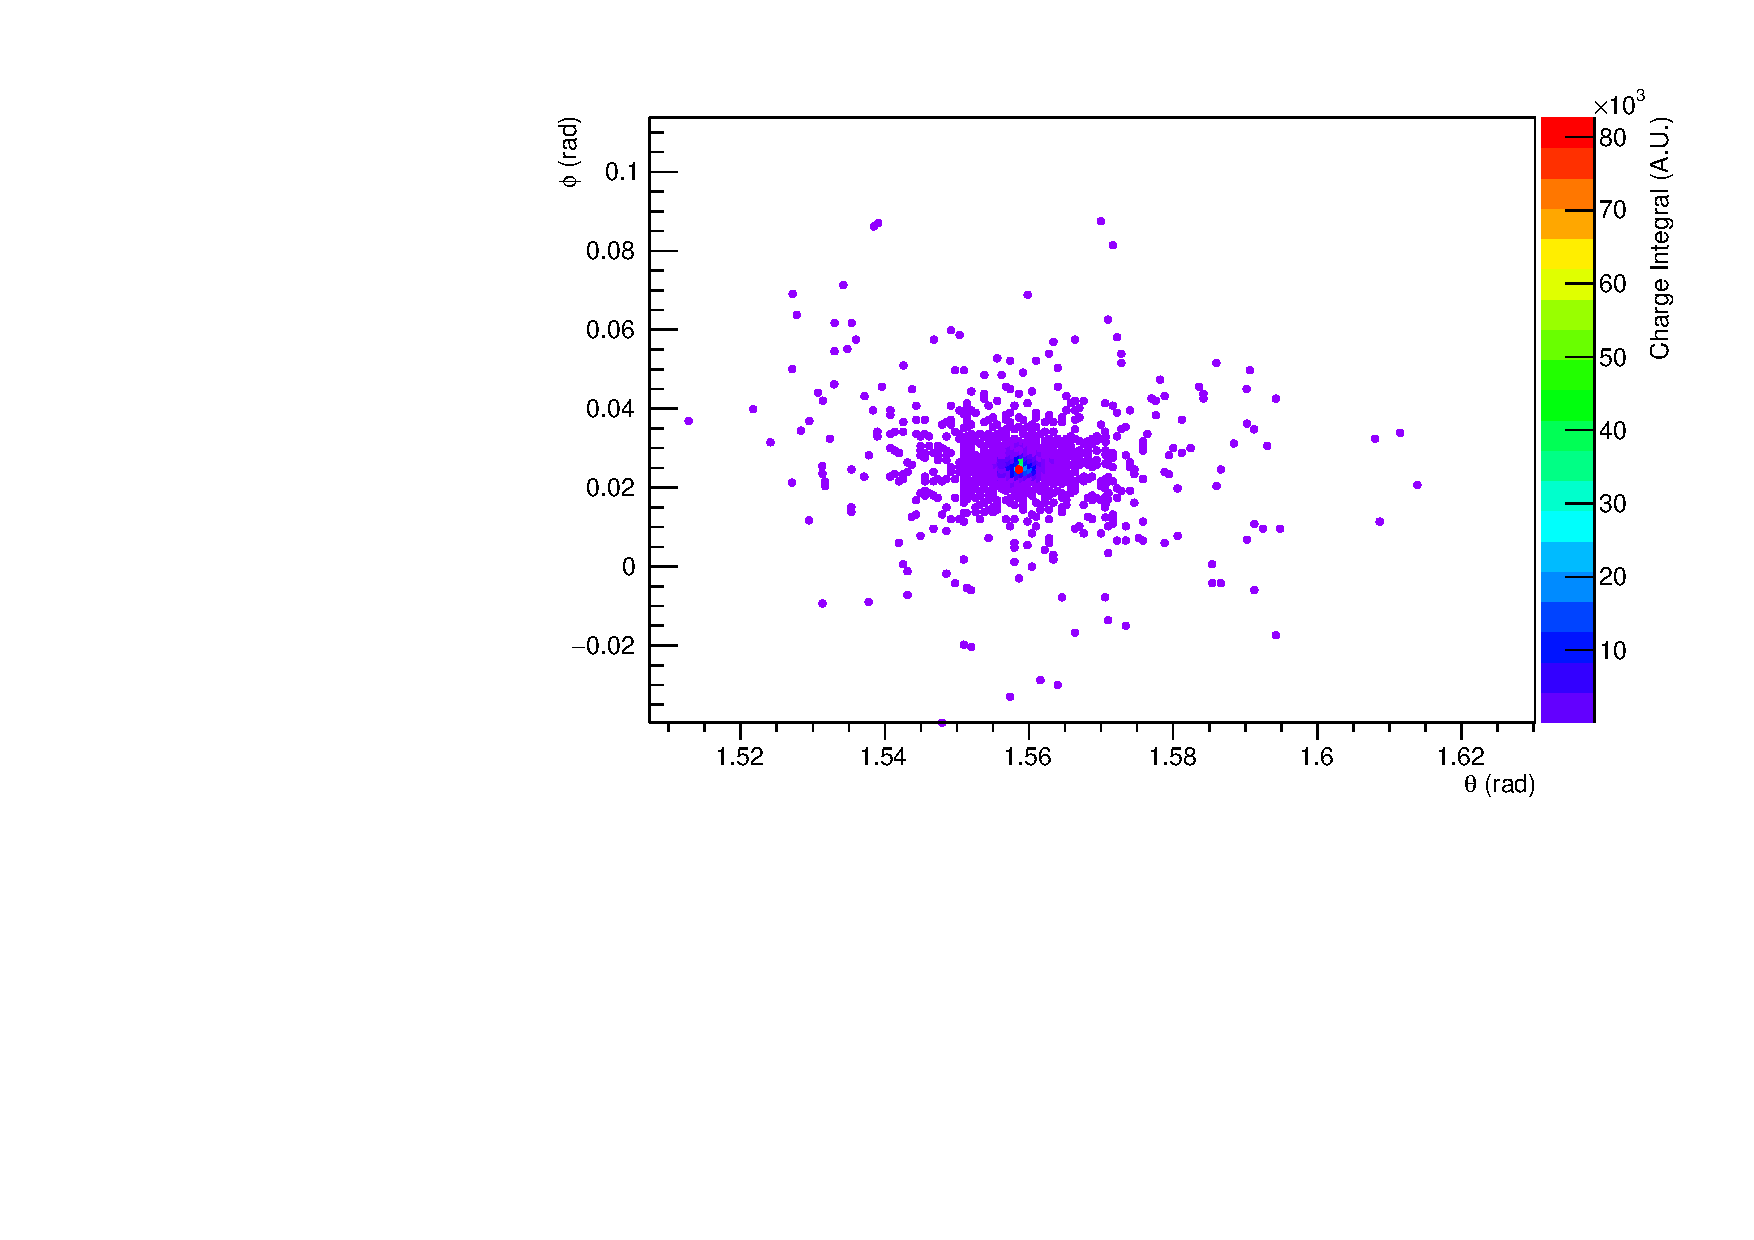
\includegraphics[width=.7\textwidth]{IMG/Cap6/Ph40GeV_ev1_scin.pdf}} \quad
	\subfloat[][$40$ GeV neutral pion.\label{fig:demo_pi}]{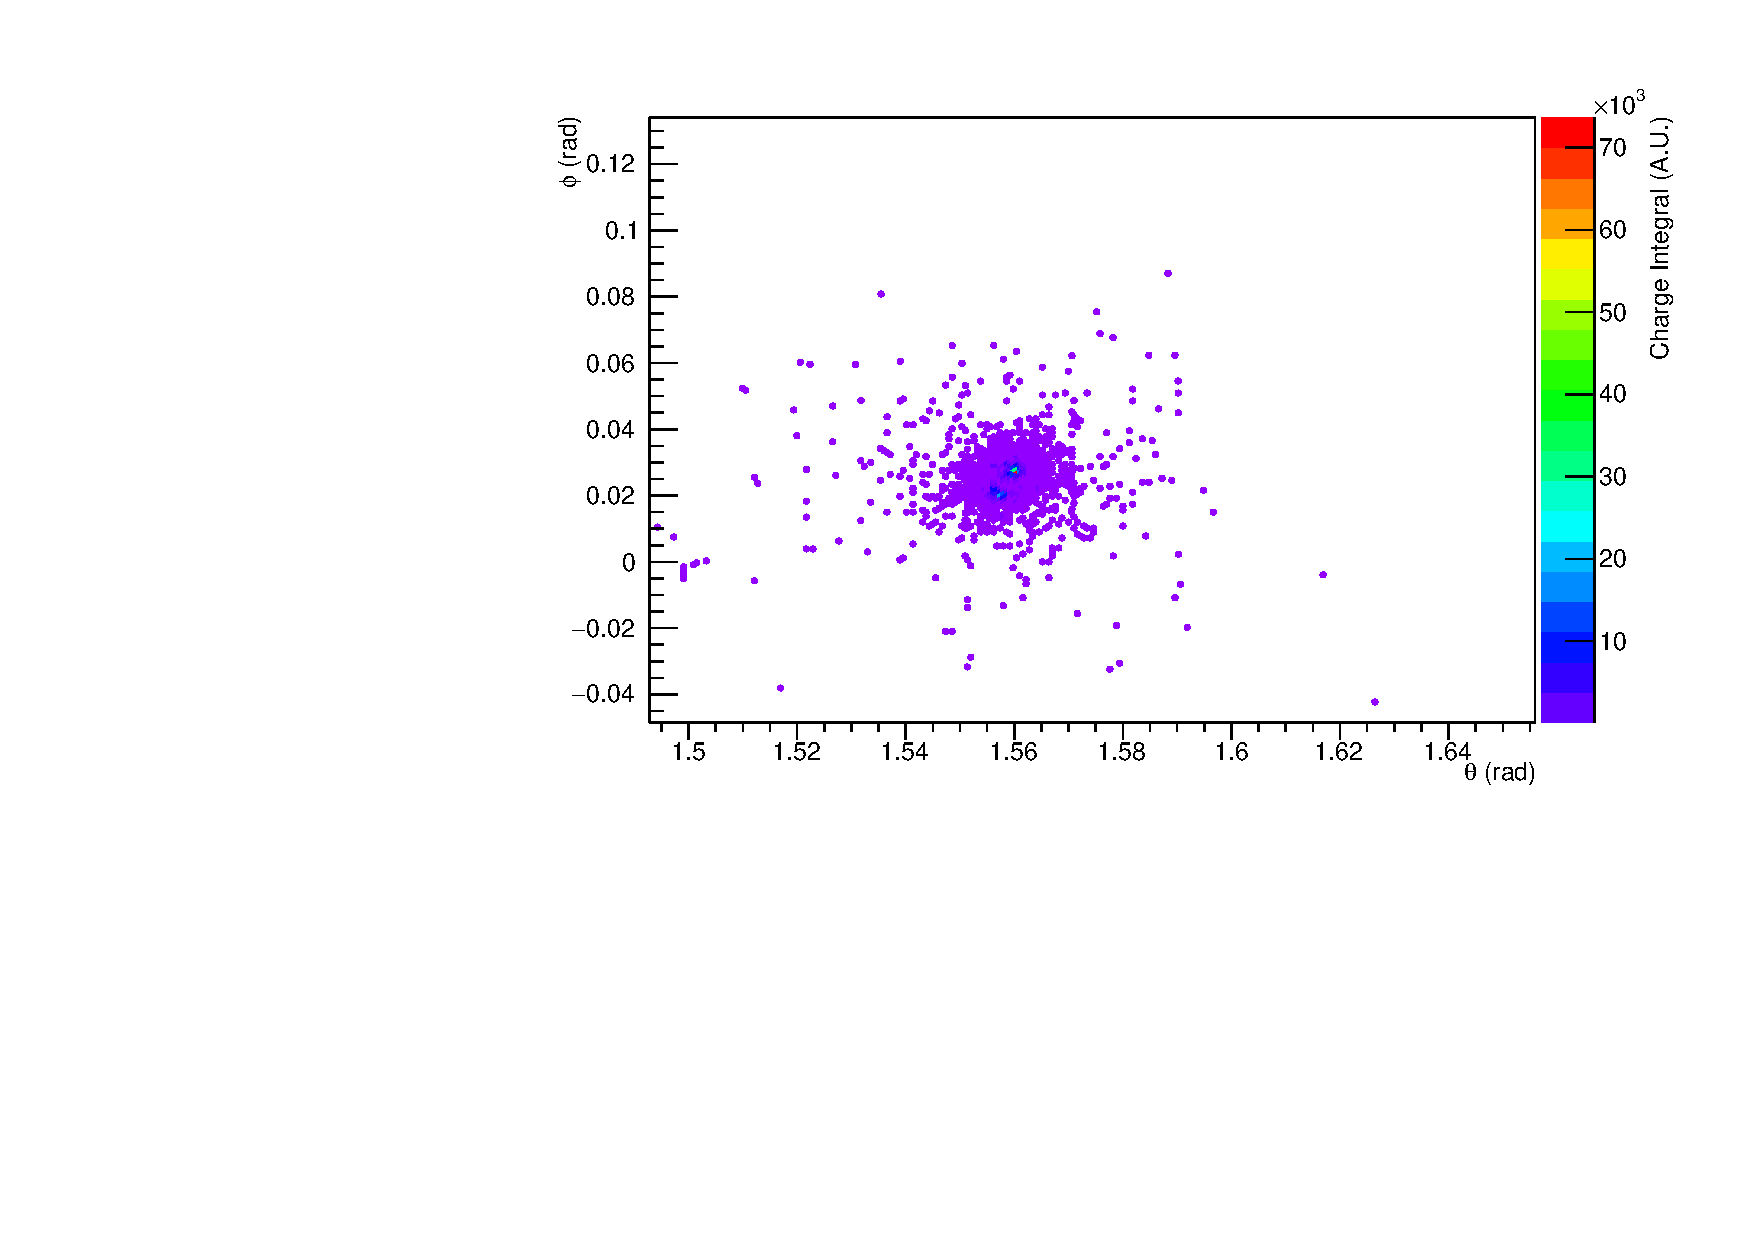
\includegraphics[width=.7\textwidth]{IMG/Cap6/Pizero40GeV_ev1_scin.pdf}}
	\caption{Spatial charge integral distributions from $\gamma$ and $\pi^0$. Each point corresponds to an activated scintillating fibre and it is represented in the $(\theta,~ \phi)$ spherical coordinates. The colour indicates the charge integral obtained from the coupled SiPM. Results form the IDEA dual-readout full simulation.}
	\label{fig:demo_shower}
\end{figure}

Usually this ID task would be performed by applying a number of filters to study the shower shape, to find the peaks of charge integral, to measure the distances between the peaks and finally establishing, with a certain probability, the final-state category and the primary-particle type. The goal is to set up a neural network able to accept data associated to such an event and make a prediction on the primary particle in a computationally effective way.\\

It is important to underline that this task is almost impossible with calorimeters presently operating at colliders due to their much coarser granularity with respect to the IDEA calorimeter.

\section{Neural Networks introduction}
Neural Networks are neural-inspired nonlinear models consisting in a group of artificial \textit{neurons} or \textit{nodes} interconnected to each other and grouped in \textit{layers}. This type of architecture is supported by a mathematical structure where each neuron has an activation degree typically ranging from $0$ to $1$ and each edge is identified by weights and biases as described in the following.\\

The simplest neural network structure follows a sequential model where neurons are grouped in \textit{layers} and linked following a sequential order, but more complex neural networks implement also loops, branching and other different flow models between layers.
The sequential model presents a first input level followed by a series of hidden levels composed by hidden neurons and then connected to the output units. A visual representation is shown in Figure \ref{fig:NN_art}.\\

\begin{figure}
	\centering
	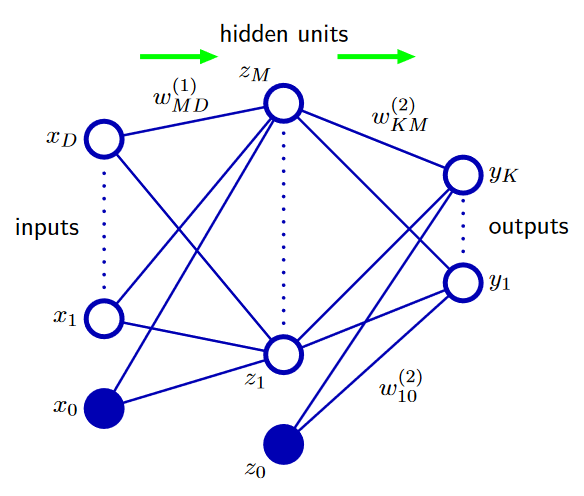
\includegraphics[width=.6\textwidth]{IMG/Cap6/NN_art.png}
	\caption{Schematic representation of a sequential model. The input, hidden, and output neurons are represented by nodes, and the weight parameters are represented by links between the nodes, for each connection the corresponding bias parameter is denoted by links coming from additional input and hidden variables $x_0$ and $z_0$. Green arrows indicate the direction of flow through the network. Figure from \cite{NN_Bishop}.}
	\label{fig:NN_art}
\end{figure}

The mathematical representation can be introduced studying a simple two-layer model. Starting from a D-dimension input vector $\bm{x}$, at the first hidden layer, for each hidden neuron, a linear combination of the input vector is calculated:
\begin{equation}
    a_j^{(1)} = \sum_{i=1}^D w_{ij}^{(1)} x_i + w_{i0}^{(1)}
\end{equation}
where $j = 1,..., M$ (M is the layer output dimension) and the matrix $\bm{W}$ is the weights matrix including biases. The quantities $a_j$ are known as \textit{activations}. On these values a $h$ nonlinear function, called \textit{activation function}, is applied:
\begin{equation}
    z_j = h(a_j^{(1)})
\end{equation}
common activation function are \textit{sigmoid}, \textit{tanh}, \textit{ReLU} (rectified linear activation unit) and \textit{Softmax} (for a description see \cite{keras_activation}). 
The obtained value are the hidden-unit neuron activation values and are used as input of the next layer. The process in the second layer is similar, evaluating, for each neuron, the following linear combinations:
\begin{equation}
    a_k^{(2)} = \sum_{j=1}^M w_{jk}^{(2)} z_j + w_{k0}^{(2)},
\end{equation}
where $k = 1,..., K$ (K is the layer output dimension), and then applying the activation function. 
In the context of the classification neural networks, the Softmax function ($S$) is a common choice. In fact this activation function normalises the sum of all the output neurons to $1$, therefore the values can be associated to the probability of classifying an event with the corresponding label:
\begin{equation}
    y_k = S(a_k^{(2)}).
\end{equation}
The whole process can be represented in a single equation for each output neuron:
\begin{equation}
    y_k = S\left(\sum_{j=1}^M w_{jk}^{(2)} h\left(\sum_{i=1}^D w_{ij}^{(1)} x_i + w_{i0}^{(1)}\right) + w_{k0}^{(2)}\right).
\end{equation}
and, to obtain a more compact expression, the values $x_0=z_0=1$ can be introduced:
\begin{equation}
    y_k = S\left(\sum_{j=0}^M w_{jk}^{(2)} h\left(\sum_{i=0}^D w_{ij}^{(1)} x_i \right) \right)
\end{equation}
making even more clear the two-layer mathematical structure.\\

Once the neural network is set up, a training process has to be performed to make the prediction effective. In order to do that, a large dataset of correctly labelled input data has to be provided. It is important to divide the dataset in at least two subsets dedicated one to the training process and one to the validation process. This separation is essential to obtain validation results that are not affected by the training process.
During the training, the elements in the weight matrix $\bm{W}$ are constantly modified to adapt the output to be as closer as possible to the correct label. These corrections are quantified by an error function that indicates the discrepancy between the output and the correct result. In classification tasks, a common error function choice is the \textit{cross-entropy} (given by the negative log likelihood):
\begin{equation}\label{eq:err_func}
    E(\bm{w}) = -\sum_{n=1}^N\sum_{k=1}^K t_{nk}\ln{y_{nk}(\bm{x}_n,\bm{w})}
\end{equation}
where $t_n$ are the target vectors and $y_n=(\bm{x}_n,\bm{w})$ are the output vectors, with a dataset dimension of $N$ and $K$ different and mutually exclusive label possibilities.\\
The ideal neural network corresponds to the one that satisfy the condition $t_{nk} = y_{nk}$ for each $n$ and $k$. Being their value bounded to be either $0$ or $1$ by the target vectors, the minimum cross-entropy value is $0$. With a non-ideal NN, the cross-entropy value increases with the worsening of the performance.\\  
The training aim is to correct weights and biases values in order to minimise the error function.\\
Once this step is completed the neural network is ready to perform predictions and classify new data.\\

The study is performed with two different neural network structures that take advantage of different layer types described in the following.

\subsection*{Dense layer}
The dense layer is the simplest and most common layer, but far from being the lightest. It is classified as a fully connected layer, meaning that each output neuron receive an input value from each input node.\\
Mathematically, this type of layer consist in a matrix application on the input vector ($\bm{v}_i$) providing an output vector ($\bm{v}_o$) after the inclusion of a bias vector ($\bm{w}_0$):
\begin{equation}
    \bm{v}_o = \bm{W}\bm{v}_i+\bm{w}_0.
\end{equation}

The layer is extremely parameter consuming, let consider a single layer that connects two group of nodes: it is common to use numbers of neuron that are powers of $2$ ($32$, $64$, $128$...). So the number of parameters associated to a single dense layer with an input dimension of $64$ and an output dimension of $32$ is:
\begin{equation*}
    64 \cdot 32 \text{(weights)} + 1 \cdot 32 \text{(biases)} = 2080.
\end{equation*}
This number can increase very rapidly with the number of neurons.\\
Being the basic type of layer, it is often used to graphically represent general neural networks, for example, Figure \ref{fig:NN_art} shows a sequence made by two consecutive dense layers.

\subsection*{Dropout layer}
Considering the extremely large number of training parameters, it is common practice to introduce the so called \textit{regularisation} techniques to increase the capability of neural networks in generalising well with new data. The use of a Dropout layer is one of them.\\
The basic idea is to reduce the spurious correlations that could occur between neurons in the network, preventing the \textit{overfitting}, a condition in which the model fits very close the training dataset but may fail in fitting unknown new data. In practical terms, the dropout layer randomly "drops out" neurons (and the corresponding connections) following a probability $p$. This process is applied in each training step. An intuitive representation is sketched in Figure \ref{fig:Drop}.

\begin{figure}
	\centering
	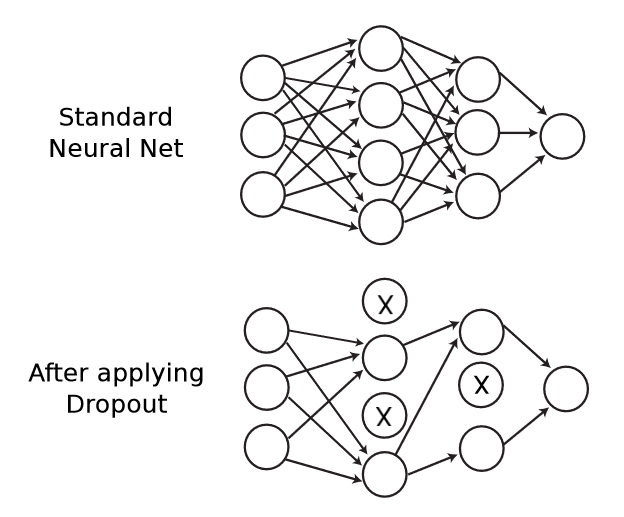
\includegraphics[width=.6\textwidth]{IMG/Cap6/Dropout.png}
	\caption{Neurons during training are randomly switched off with a probability $p$. A lighter network is produced reducing correlations between nodes. Figure from \cite{ML4ph}.}
	\label{fig:Drop}
\end{figure}

\subsection*{Conv2D layer}
A useful layer in image processing is the convolution layer. It identifies a category of NN called Convolutional Neural Networks (CNNs).\\
A convolution consists in a simple application of a filter to an input that results in an activation. The application of the same filter repeatedly to the same input results in a map of activations called a feature map. It indicates the locations of a detected feature (and its intensity) in an input image.\\
Figure \ref{fig:Conv2D} represents the application of a filter or kernel ($K$) over an input matrix ($I$). As it can be seen, the feature map is composed considering all the sub-images with the same size of the kernel; each sub-image is associated to an activation value obtained through the formula:
\begin{equation}
    a = \sum_{i = 1}^{D_K}\sum_{j = 1}^{D_K} I_{i,j} \cdot K_{i,j} + b
\end{equation}
where $D_K$ is the dimension of the kernel, typical values are $1\times 1$, $3\times 3$, $5\times 5$, and $b$ is the bias value. An activation is obtained from each sub-image and then corrected by the activation function. These outputs compose the feature map.\\
The layer output is a group of feature maps obtained from different filters. The number of filters evaluated represents the capability of the layer to identify different patterns.\\

In terms of trainable parameters, a convolution layer with $32$ kernels of $3\times3$ size is lighter then a dense one:
\begin{equation*}
    9\cdot 32 \text{(weights)} + 1 \cdot 32 \text{(biases)} = 320.
\end{equation*}

\begin{figure}
	\centering
	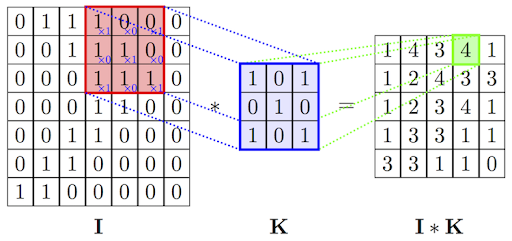
\includegraphics[width=.6\textwidth]{IMG/Cap6/ConvScheme.png}
	\caption{Example of convolution applying a single kernel $K$ on the input matrix $I$. The red square is the sub-image considered and convoluted with the blue matrix giving the activation value in the green box. The procedure is done over all the sub-images producing the feature map on the far right.}
	\label{fig:Conv2D}
\end{figure}

\subsection*{MaxPool2D layer}
A natural next-step to the convolution layer is represented by the category of pooling layers. This type of layers has the aim of reducing the size of the activation maps.\\
In particular, a MaxPool2D layer considers a sub-matrix with a fixed size, typically $2\times2$ or $3\times3$, and records the max value. By performing the process over all the input sub-matrices, the result is a smaller output matrix that keeps the geometrical feature informations. A pictorial representation of the layer is shown in Figure \ref{fig:MaxPool}.

\begin{figure}[b]
	\centering
	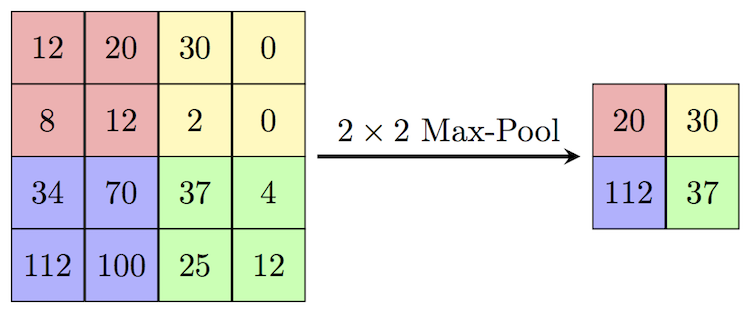
\includegraphics[width=.6\textwidth]{IMG/Cap6/MaxpoolSample2.png}
	\caption{MaxPool2D effect sketched where the same colour represents the sub-matrix considered and the corresponding output.}
	\label{fig:MaxPool}
\end{figure}

%\subsection*{GlobalAveragePooling2D layer}

\subsection*{VGGNet structure} \label{subsec:VGGNet_teo}
The VGGNet structure is a neural network concept introduced in 2015 in the article "Very Deep Convolutional Networks for Large-Scale Image Recognition" \cite{VGGArt} (the name VGG is the acronym for Visual Geometry Group, their lab in Oxford).\\
The proposed, and then accepted as a standard, powerful structure is composed by several small-size filter chains (i.e. kernel size of $1\times1$ or $3\times3$) and max pooling with size of $2\times2$ is used after most, but not all, the convolutional layers. The idea is that consecutive small-size filters approximate larger filter effects with an higher number of parameters. Another important characteristic is the large number of filters used: typically a deeper layer has a greater number of kernels starting from, at least, $32$.\\
In Figure \ref{fig:VGG_table}, the structures studied in \cite{VGGArt} are listed where groups of two or three convolutional layers are followed by max pooling ones and, at the end, the last max pooling layer output is flattened and used as input for a group of dense layers till the classification.\\

\begin{figure}
	\centering
	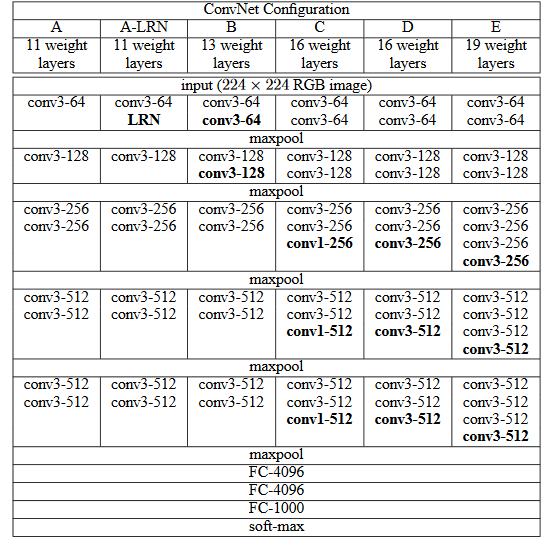
\includegraphics[width=.8\textwidth]{IMG/Cap6/VGG_art.png}
	\caption{Schematic representation of CNN structures studied by Karen Simonyan and Andrew Zisserman. Each column correspond to a CNN with different depth increasing from the left (A) to the right (E), as more layers are added (the added layers are shown in bold). The convolutional layer parameters are denoted as “conv[receptive field size]-[number of channels]". Image from  \cite{VGGArt}.}
	\label{fig:VGG_table}
\end{figure}

A VGGNet like structure has been set up and used to perform the task of $\pi^0/\gamma$ discrimination and will be described in detail in Paragraph \ref{sec:NN_perf}. A schematic representation of the structure in our context is shown in Figure \ref{fig:VGG_our_scheme}.

\begin{figure}
	\centering
	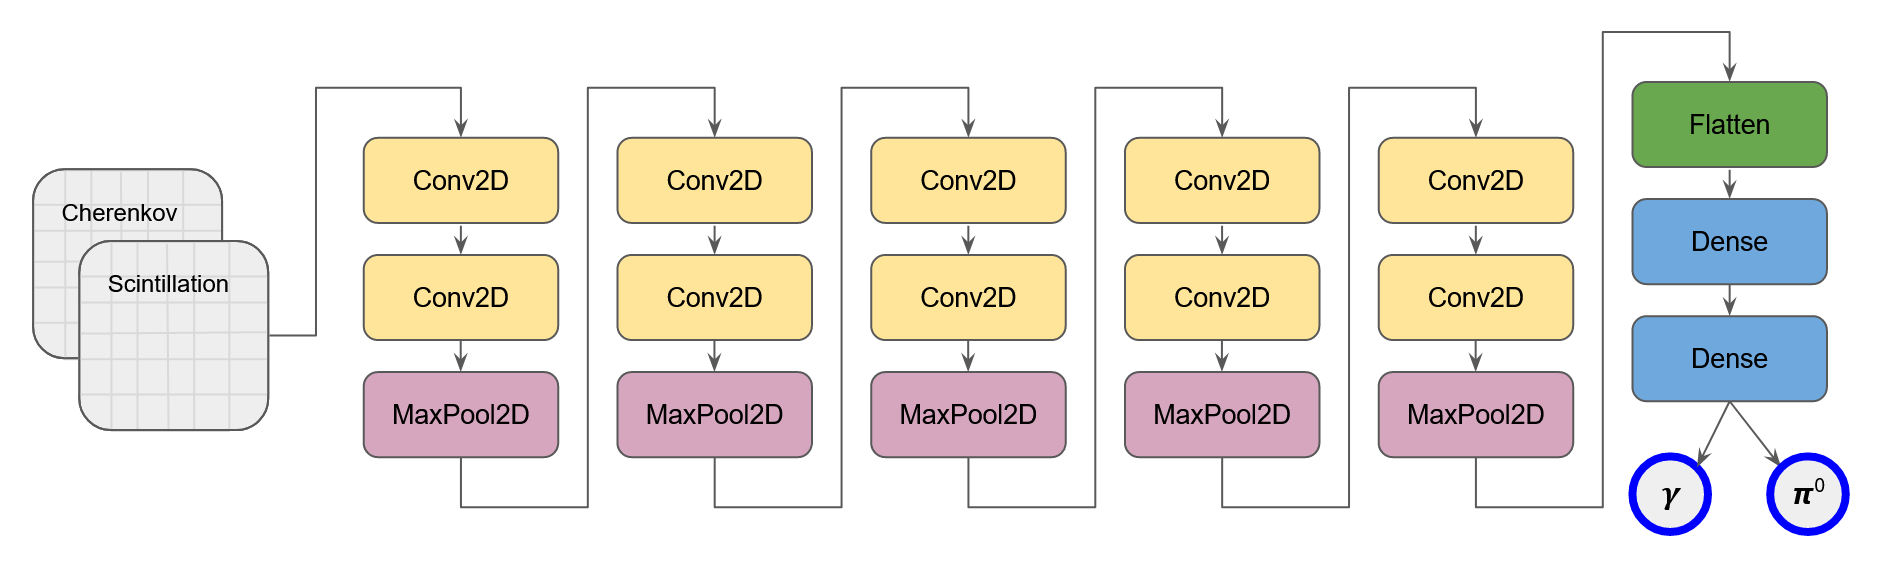
\includegraphics[width=.8\textwidth]{IMG/Cap6/VGG_our_scheme.png}
	\caption{Schematic representation of the VGG Network used in our task.}
	\label{fig:VGG_our_scheme}
\end{figure}

\subsection*{ResNet structure} \label{subsec:ResNet_teo}
Residual Networks, or ResNet, are another innovative concept of CNN introduced in 2016 in the article "Deep Residual Learning for Image Recognition" by Kaiming He et al. \cite{ResNetArt}.\\
The structure is composed as a plain convolutional network with small kernel size (same as in VGGNet) and the sequence of convolutional  layers is splitted in several \textit{residual} blocks. The innovative aspect is that the input of each block is the sum of the input and the output of the previous block; in this way the connection between layers is no more sequential due to the fact that some of the connections skip hidden layers% as in the schematic path
. The structure and flow of data are shown in Figure \ref{fig:ResNet_scheme}, where two different ResBlock are sketched.\\

\begin{figure}
	\centering
	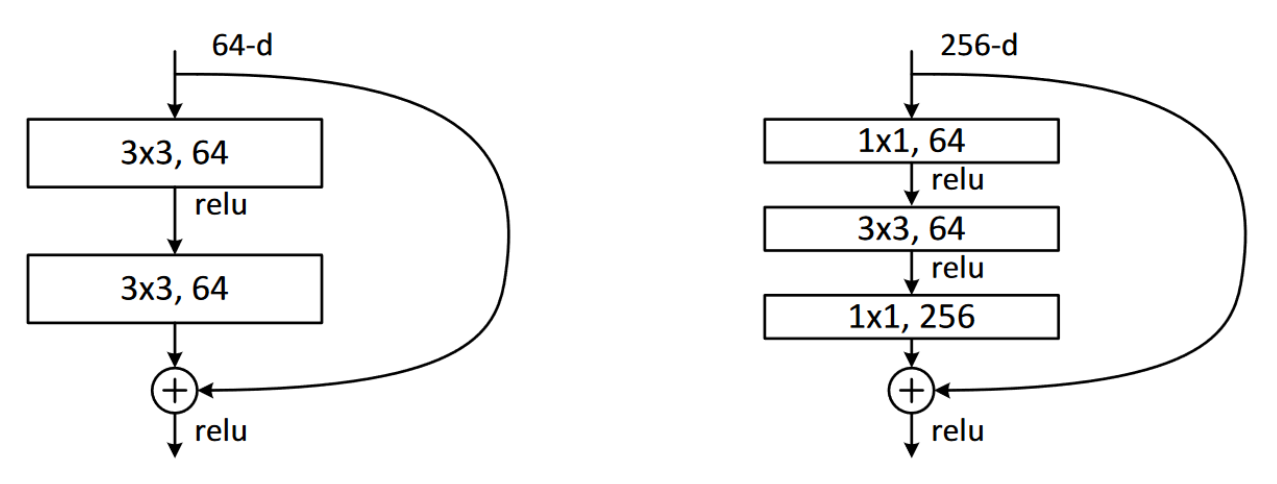
\includegraphics[width=.7\textwidth]{IMG/Cap6/ResNet_scheme.png}
	\caption{Schematic representation of residual blocks with arrows to indicate the data flow. On the left, a simple two convolutional blocks, on the right, a "bottleneck" building block. Figure from \cite{ResNetArt}.}
	\label{fig:ResNet_scheme}
\end{figure}

The last block is followed by an average pooling layer (similar to the max pooling layer, but it records the average value and not the max value) and then a structure of consecutive dense layers till the classification one, with Softmax as activation function.\\

A ResNet like structure has been set up and used to perform the task of $\pi^0/\gamma$ discrimination and to compare the result with VGGNet. It will be described in detail in Paragraph \ref{sec:NN_perf}. A schematic representation of this structure in our context in shown in Figure \ref{fig:Res_our_scheme}.

\begin{figure}
	\centering
	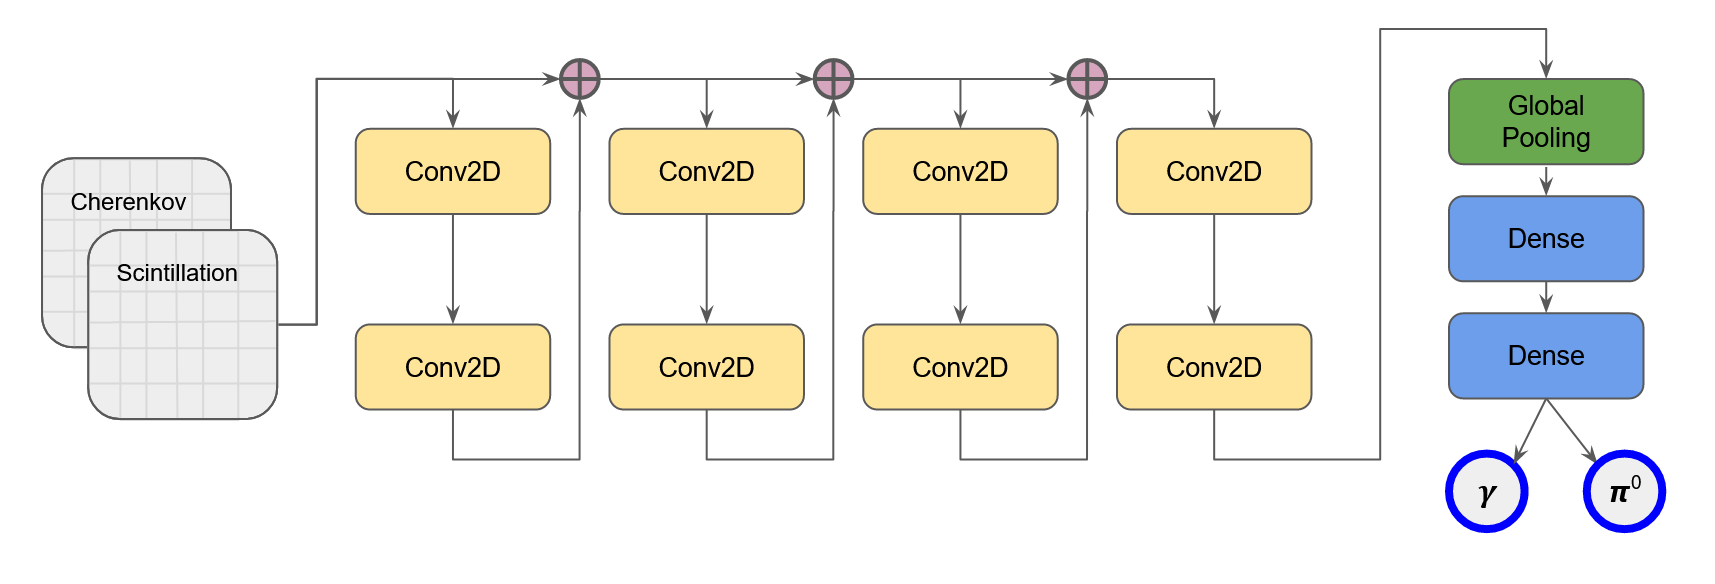
\includegraphics[width=.8\textwidth]{IMG/Cap6/Res_our_scheme.png}
	\caption{Schematic representation of the Residual Network used in our task.}
	\label{fig:Res_our_scheme}
\end{figure}

\section{Data preparation}\label{sec:NN_data}
The data are produced with the IDEA DR Calorimeter full simulation, neutral pions and photons are fired from the interaction point to tower $1$ of the calorimeter. In the first step, photons and neutral pions with fixed energy of $40$ GeV are simulated.\\
The simulation input data used for this study are:
\begin{itemize}
    \item spatial coordinates of the fibre inner tip $(x, y, z)$%(considering the inner tip)%
    ;
    \item fibre type (Cherenkov or scintillating);
    \item charge integral from the SiPM digitization software.
\end{itemize}
The typical coordinate system for a $4\pi$ calorimeter is the spherical one so the cartesian coordinates have been transformed in spherical ones. Then, at each $(x, y, z)$ point, the charge integral has been associated to a point in the $(\theta,\phi)$ space. Finally, the input data are grouped in two subsets by filtering with respect to the fibre types. The results obtained can be plotted in a 3D-graph to visually check the effective correctness of the process. An event display can be seen in Figure \ref{fig:3Dgraph}.

\begin{figure}
	\centering
	\subfloat[][Cherenkov signal.]{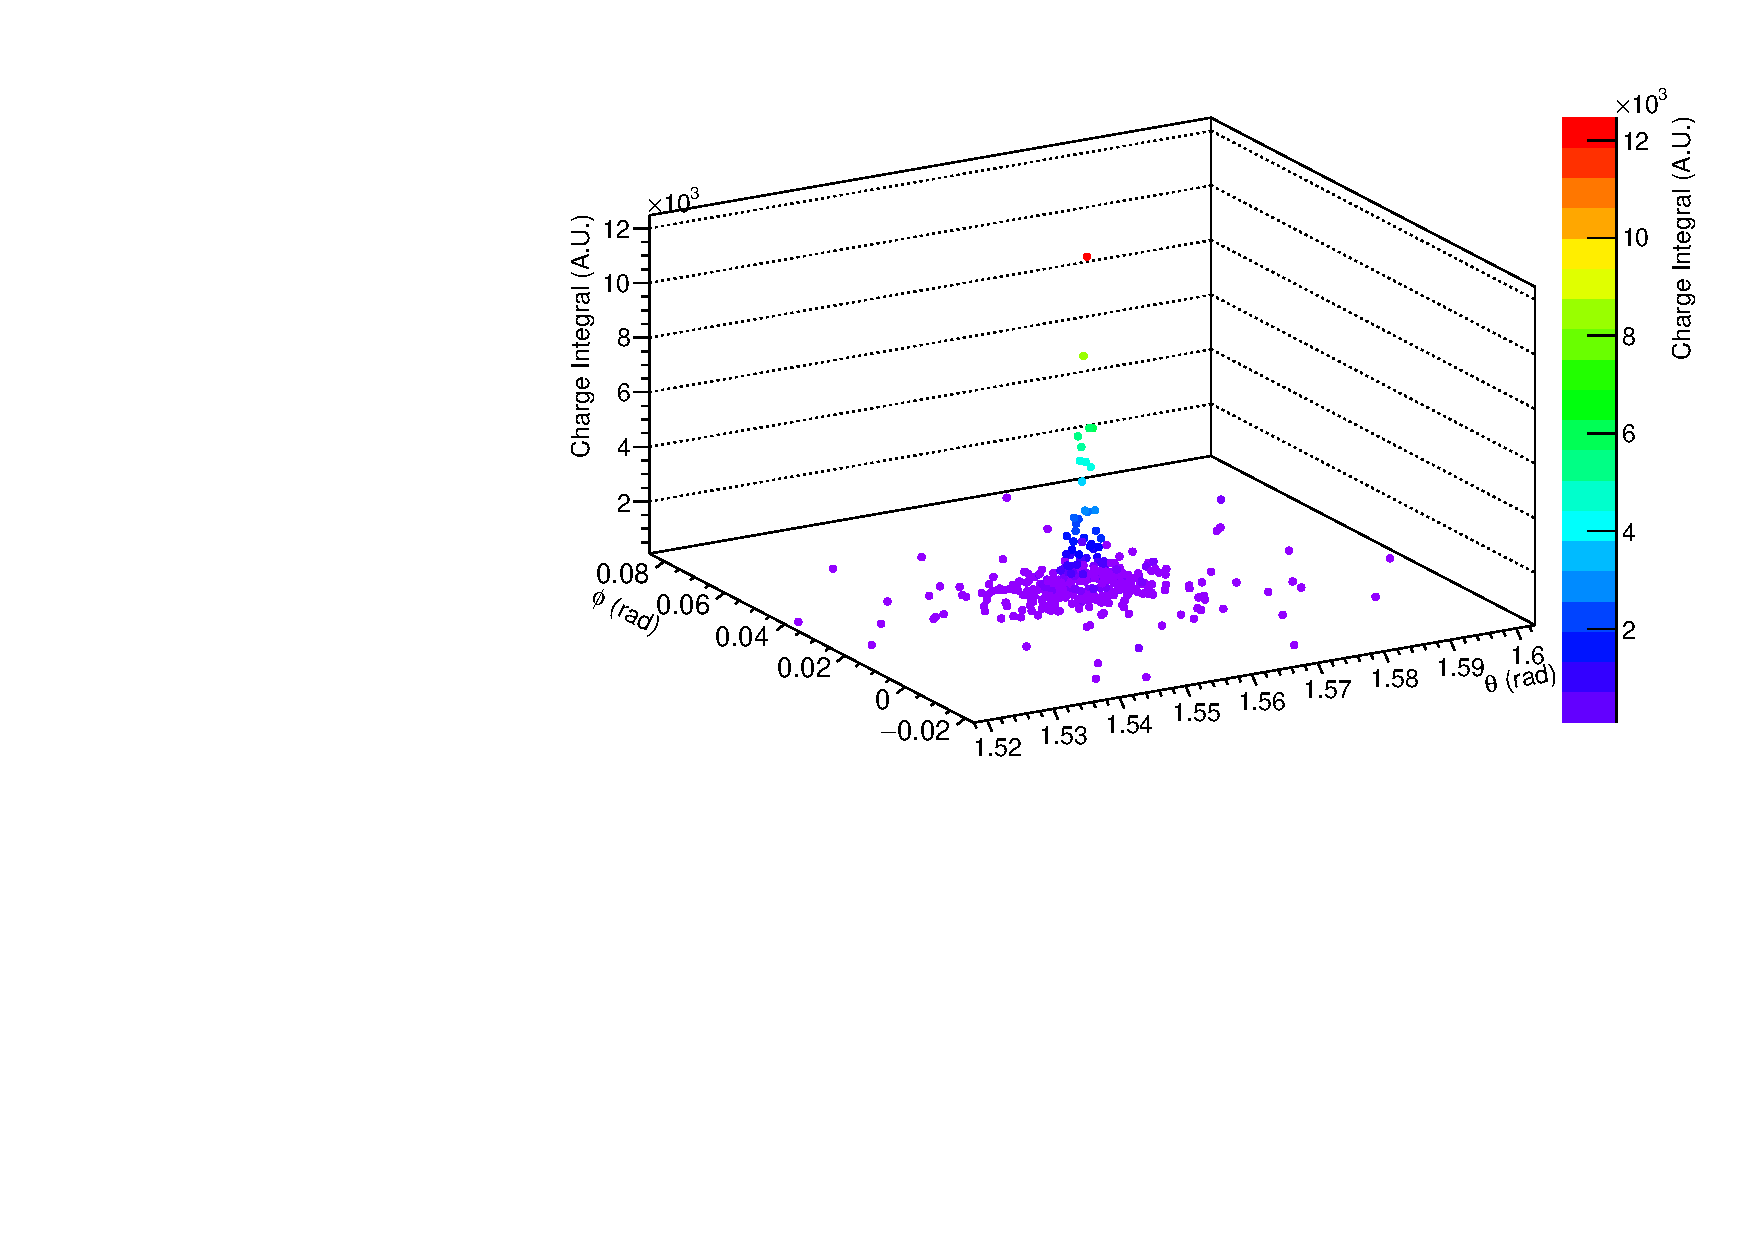
\includegraphics[width=.45\textwidth]{IMG/Cap6/Ph40GeV_ev15_cher_TGraph3D.pdf}} \quad
	\subfloat[][Scintillation signal.]{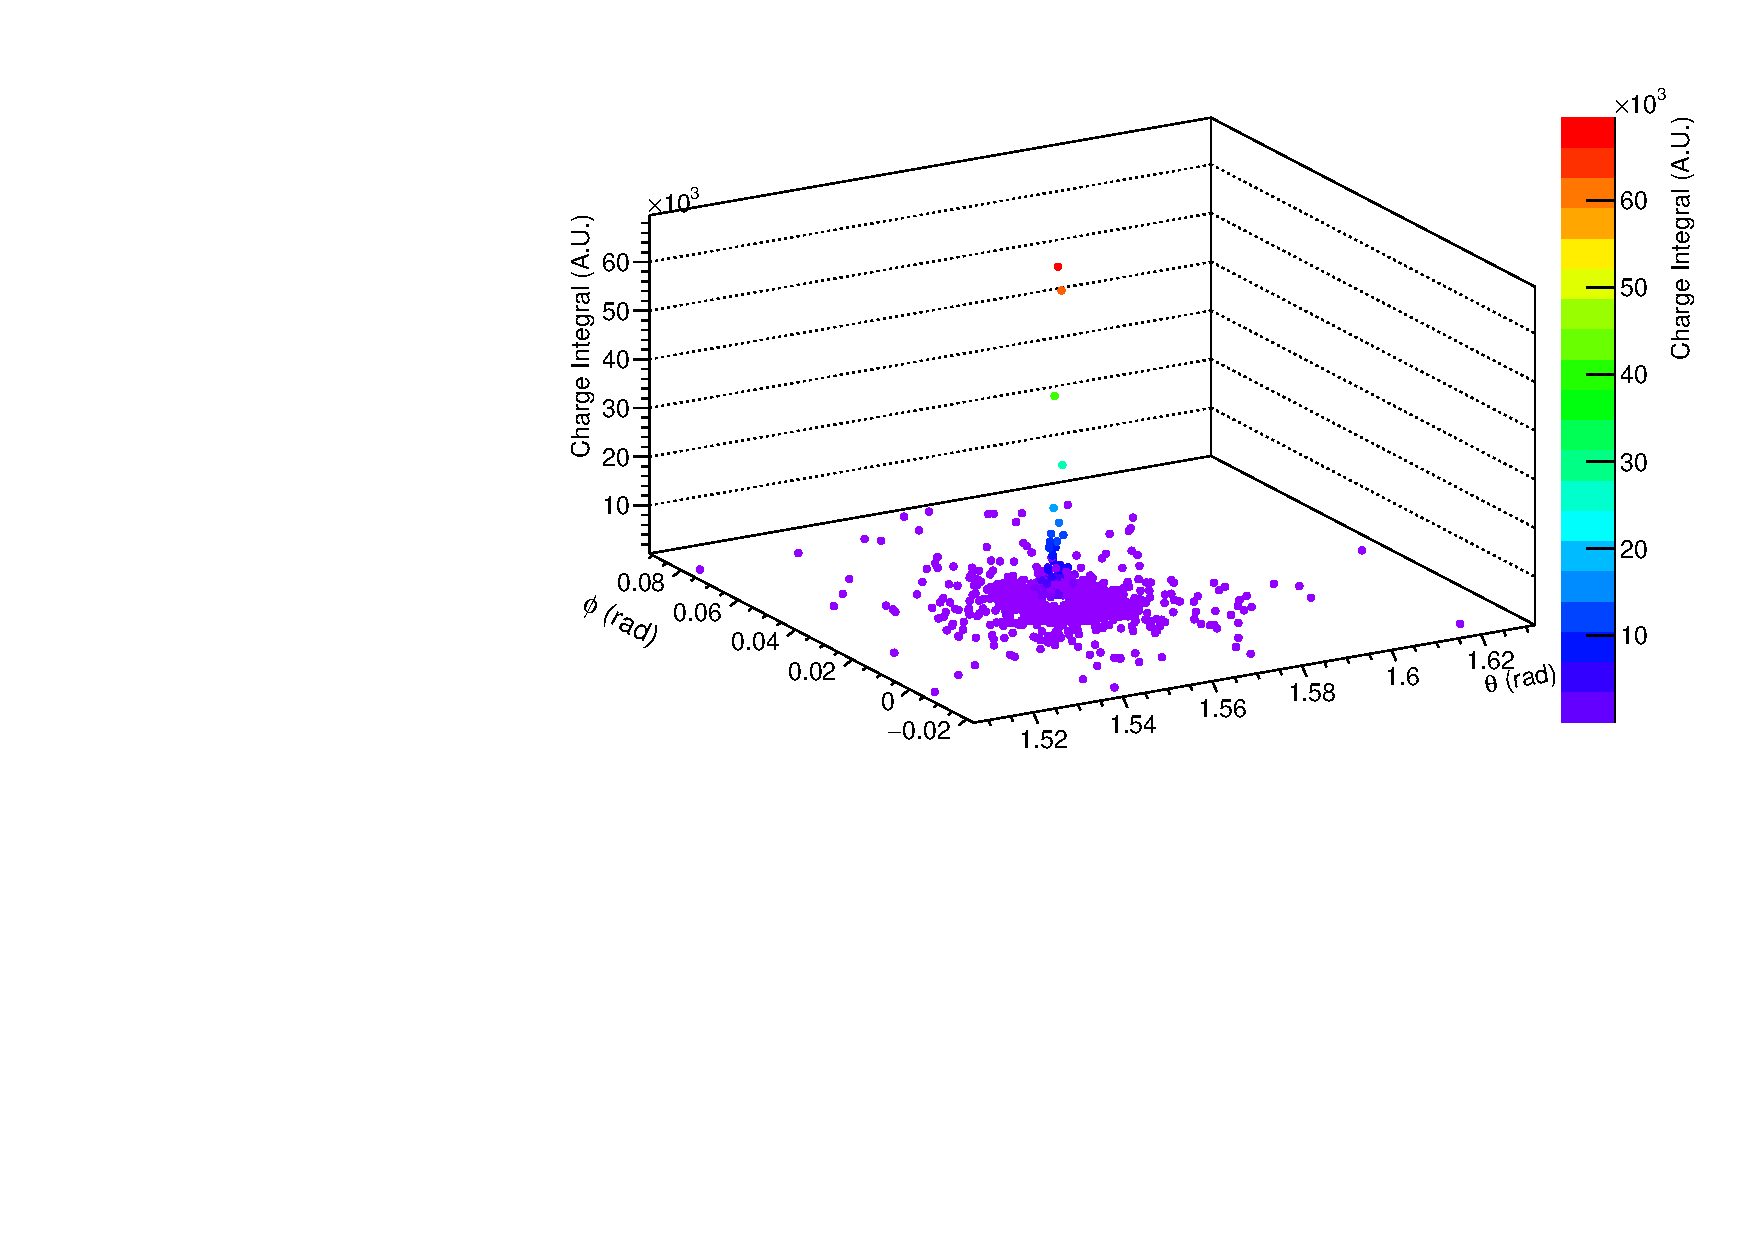
\includegraphics[width=.45\textwidth]{IMG/Cap6/Ph40GeV_ev15_scin_TGraph3D.pdf}}
	\caption{3D-graphs representing Cherenkov and scintillation signals from the same simulated event (with a $40$ GeV photon as primary particle).}
	\label{fig:3Dgraph}
\end{figure}

To feed the CNNs, the dataset has to be properly prepared. The input for the VGGNet and the ResNet has to be a dimension-fixed matrix. Every event will be characterized by two features (Cherenkov integral and scintillation integral), each one represented by a grid reproducing the spatial distribution of the data.
The squared area of interest in the  ($\theta$,$\phi$) space has been selected (in radians) as $(1.51,1.63)$, along $\theta$, and $(-0.02,0.10)$, along $\phi$.
Different values of the grid step within this area have been compared by searching a compromise between grid shape efficiency and imaging resolution. A grid step of $0.0009$ rad for both axes, corresponding to a single fibre per bin, has been selected. The grid can be represented as a 2D-histogram where the total charge integral in each bin is the bin height. (Figure \ref{fig:2Dhist} shows the histograms obtained from the same data as in Figure \ref{fig:3Dgraph}).\\
Hence the input matrix for each event has a dimension of $133 \text{ (height) }\times 133\text{ (width) }\times 2\text{ (features)}$. A 2D visualisation can be seen in Figures \ref{fig:2Dvision1}, \ref{fig:2Dvision2}, \ref{fig:2Dvision3} and  \ref{fig:2Dvision4}.\\

\begin{figure}
	\centering
	\subfloat[][Cherenkov signal.]{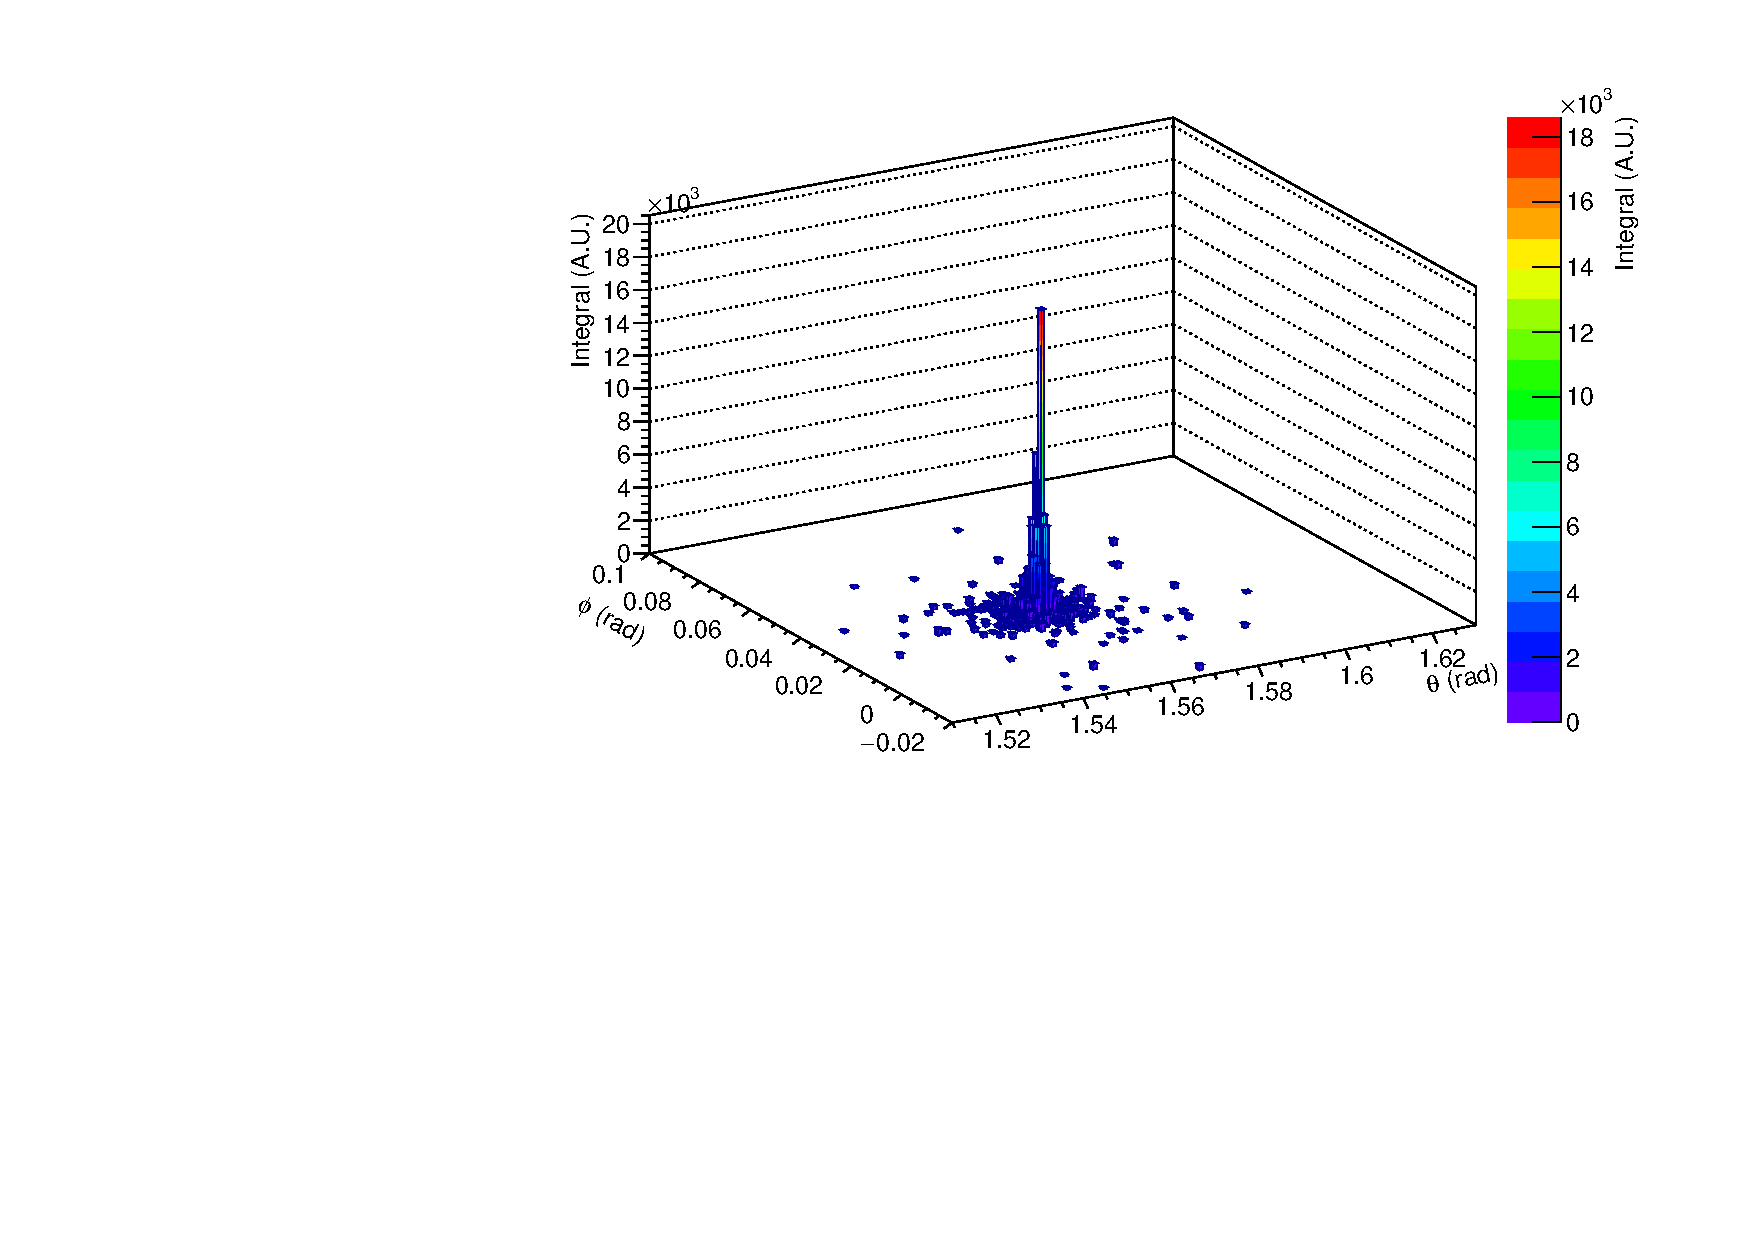
\includegraphics[width=.45\textwidth]{IMG/Cap6/Ph40GeV_ev15_cher_hist_3D.pdf}} \quad
	\subfloat[][Scintillation signal.]{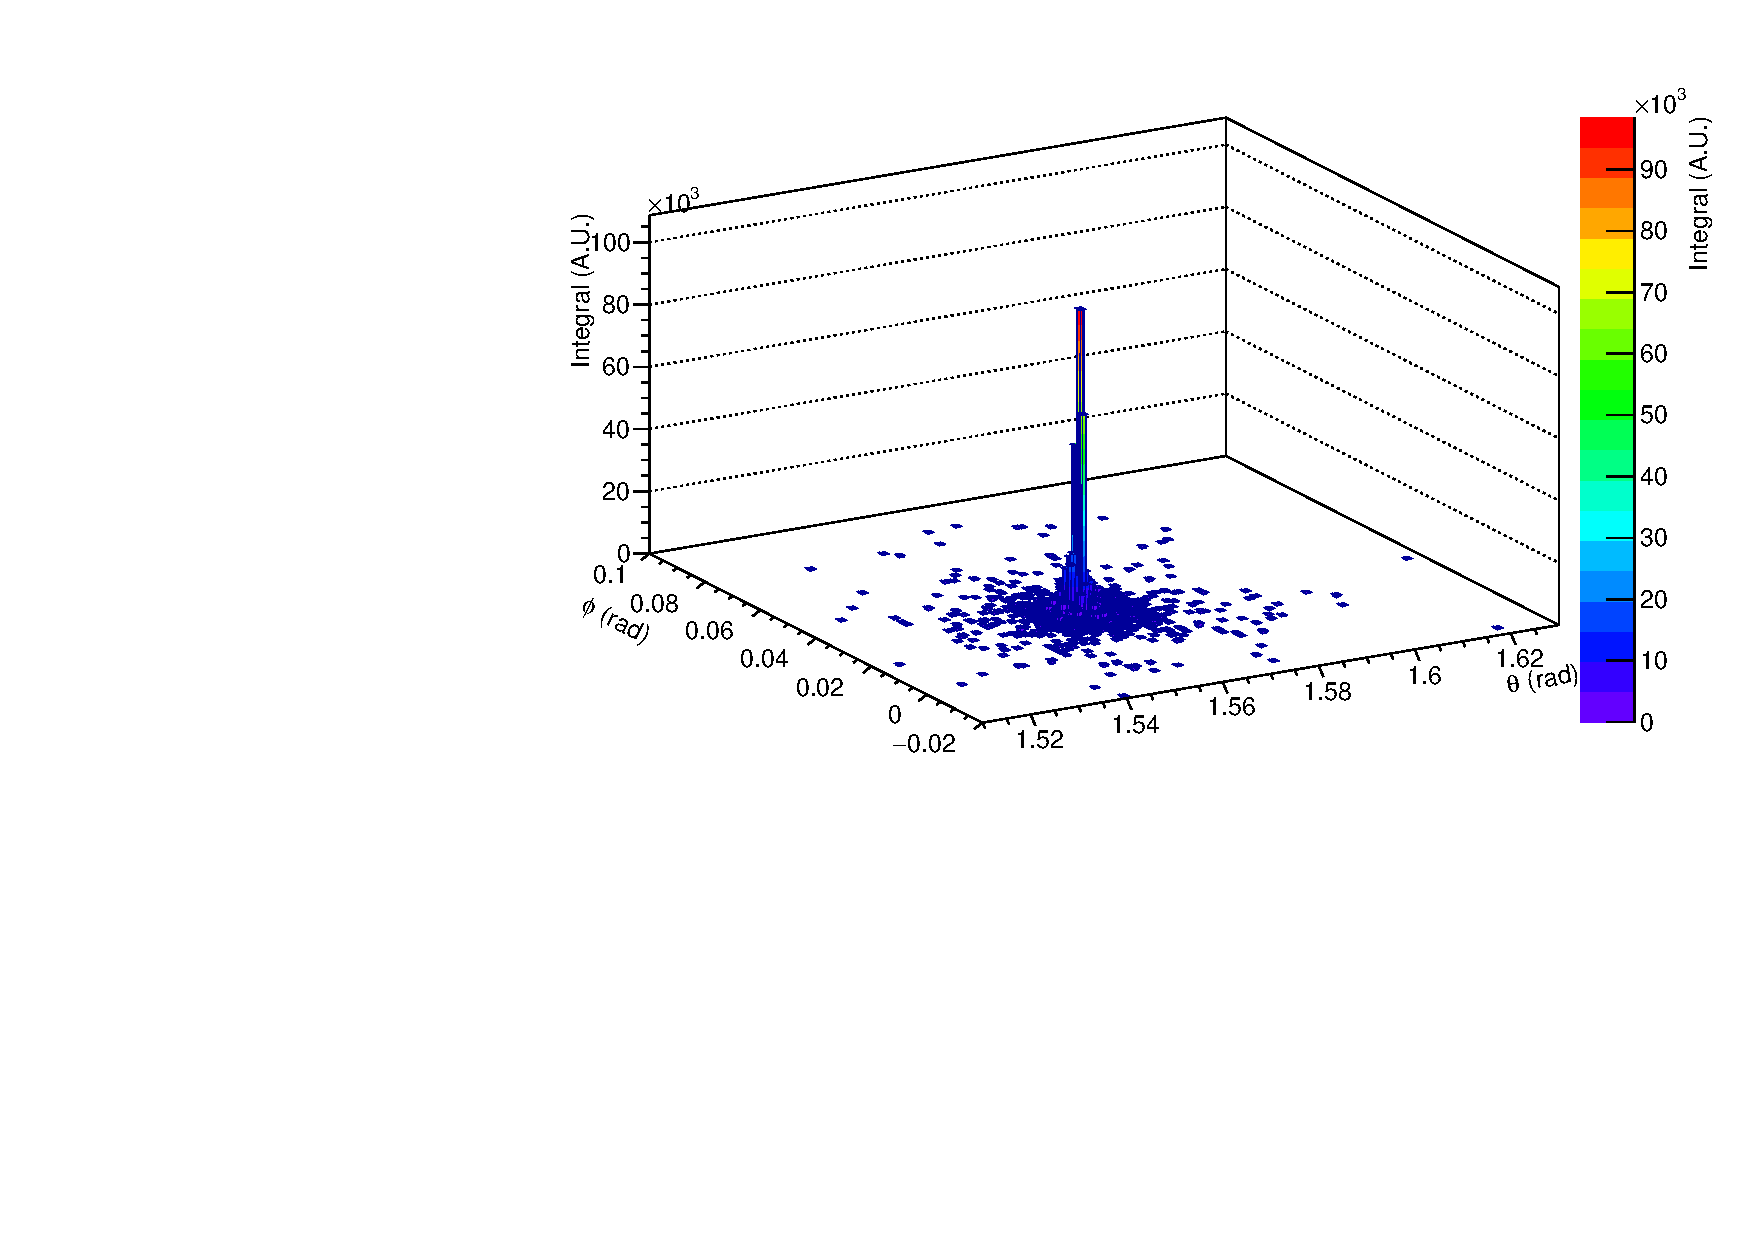
\includegraphics[width=.45\textwidth]{IMG/Cap6/Ph40GeV_ev15_scin_hist_3D.pdf}}
	\caption{2D-histograms representing Cherenkov and scintillation signals from the same sample event ($40$ GeV photon as primary particle).}
	\label{fig:2Dhist}
\end{figure}

\begin{figure}
	\centering
	\subfloat[][Cherenkov signal pre data setup.]{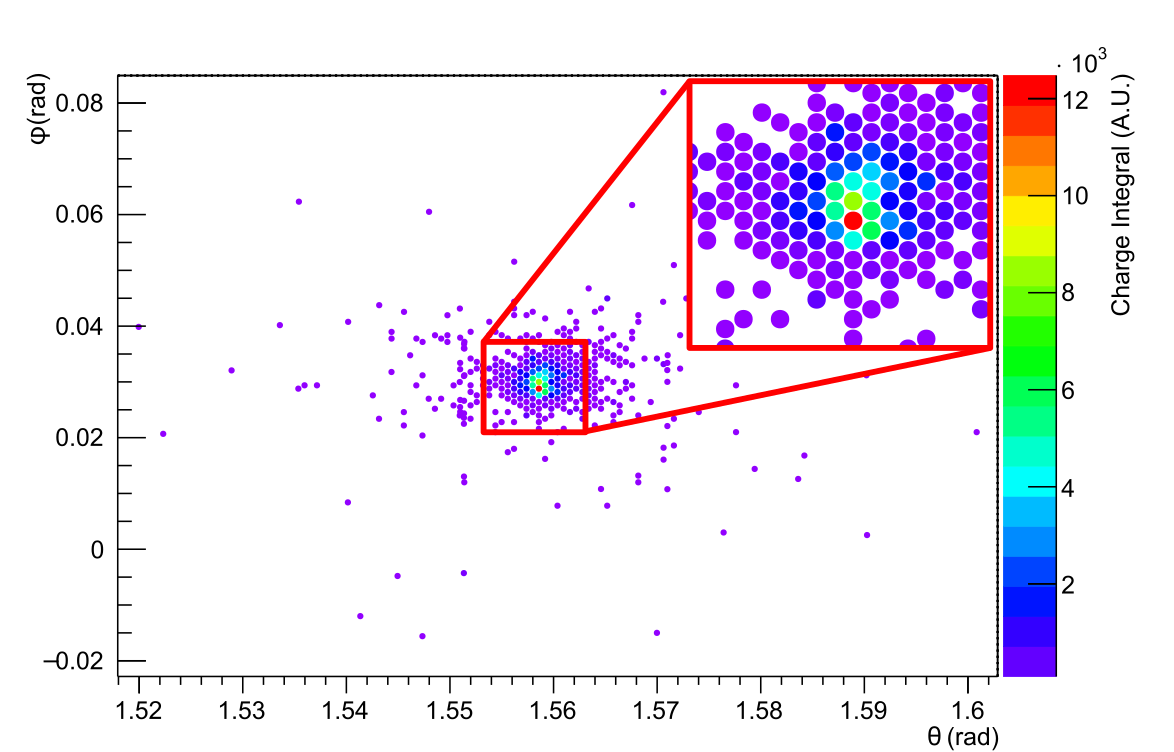
\includegraphics[width=.8\textwidth]{IMG/Cap6/Ph40GeV_ev1_cher_TGraph_flat_zoom.png}} \quad
	\subfloat[][Scintillation signal pre data setup.]{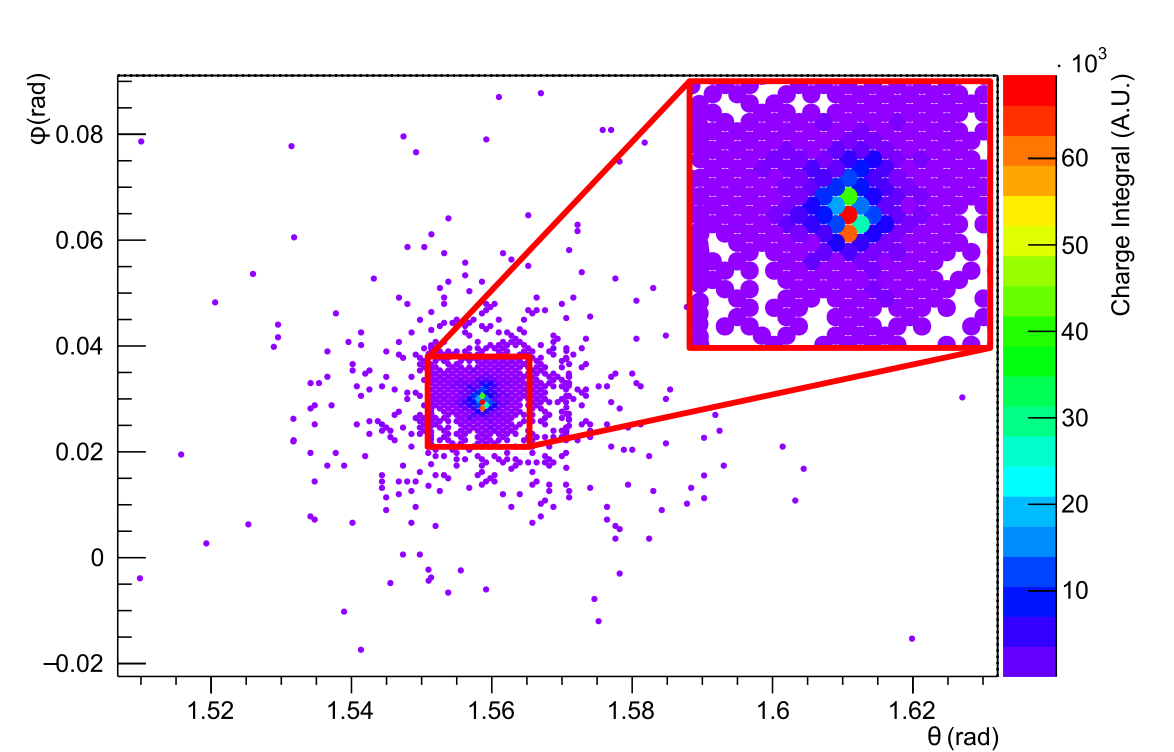
\includegraphics[width=.8\textwidth]{IMG/Cap6/Ph40GeV_ev1_scin_TGraph_flat_zoom.png}} \\
	\caption{2D-vision of data before data preparation. Data from a $40$ GeV photon.}
	\label{fig:2Dvision1}
\end{figure}
\begin{figure}
	\centering
	\subfloat[][Cherenkov signal post data setup.]{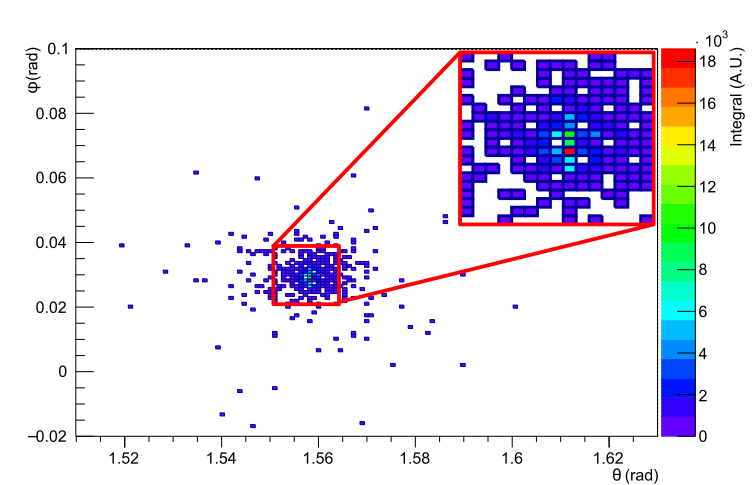
\includegraphics[width=.8\textwidth]{IMG/Cap6/Ph40GeV_ev15_cher_hist_flat_zoom.png}} \quad
	\subfloat[][Scintillation signal post data setup.]{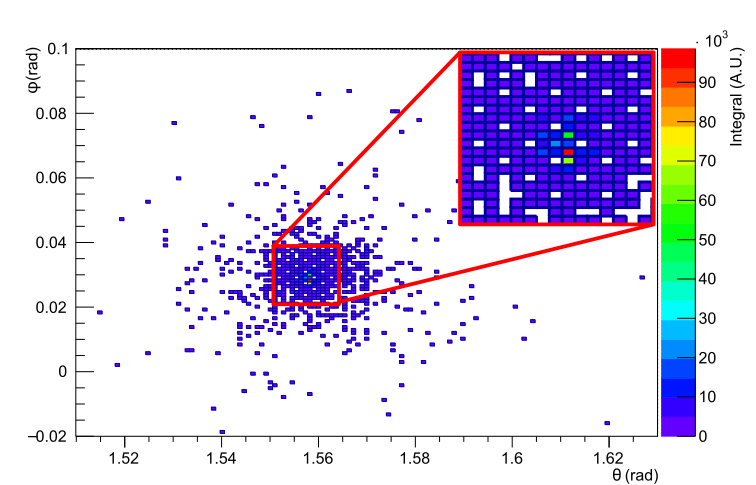
\includegraphics[width=.8\textwidth]{IMG/Cap6/Ph40GeV_ev15_scin_hist_flat_zoom.png}}
	\caption{2D-vision of data after data preparation. Data from a $40$ GeV photon.}
	\label{fig:2Dvision2}
\end{figure}
\begin{figure}
	\centering
	\subfloat[][Cherenkov signal pre data setup.]{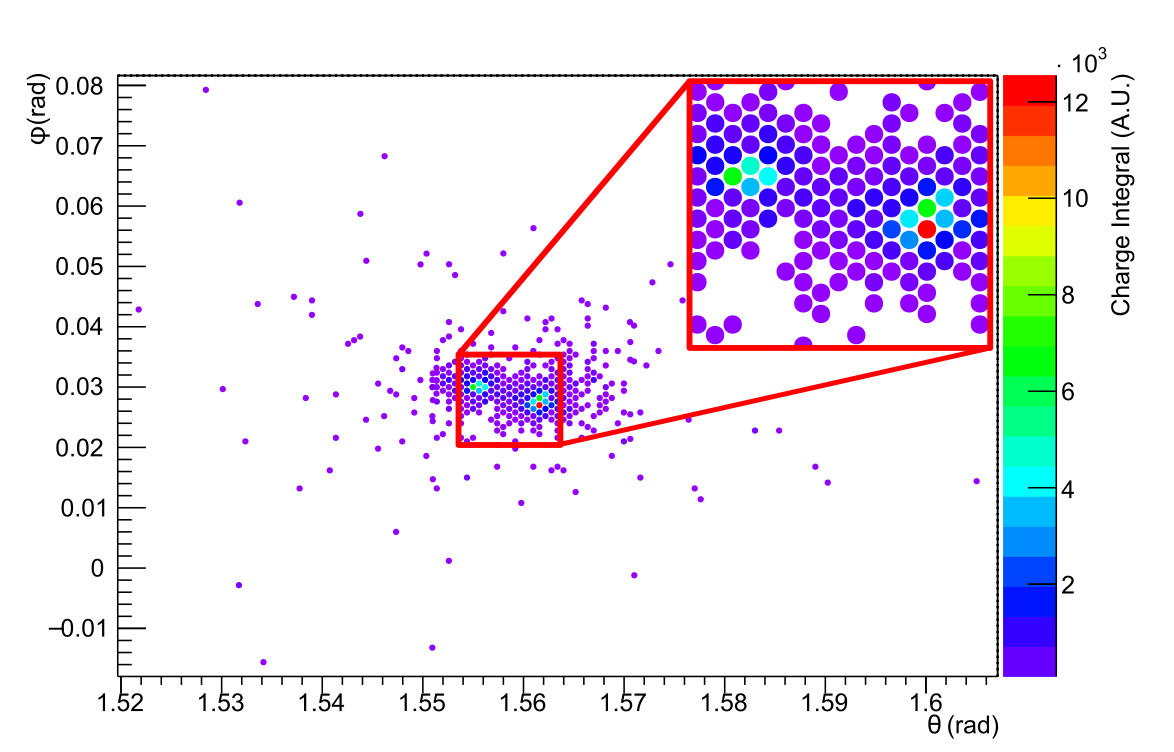
\includegraphics[width=.8\textwidth]{IMG/Cap6/Pizero40GeV_ev15_cher_TGraph_flat_zoom.png}} \quad
	\subfloat[][Scintillation signal pre data setup.]{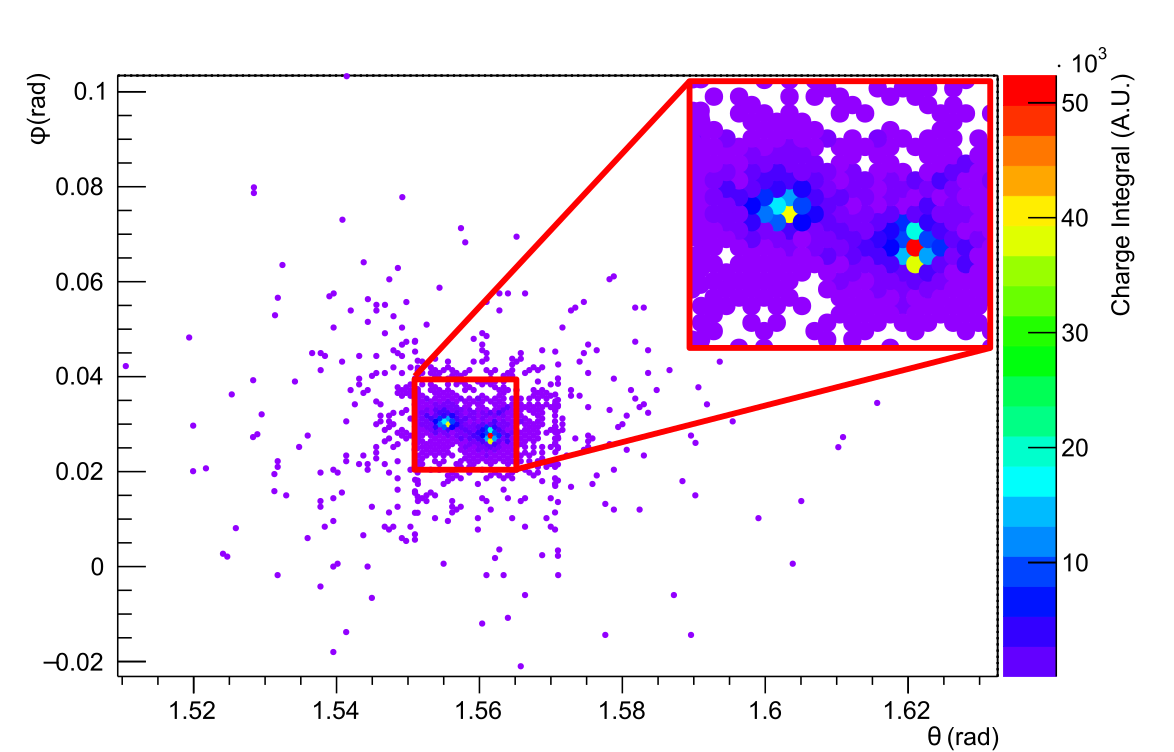
\includegraphics[width=.8\textwidth]{IMG/Cap6/Pizero40GeV_ev15_scin_TGraph_flat_zoom.png}} \\
	\caption{2D-vision of data before data preparation. Data from a $40$ GeV pion.}
	\label{fig:2Dvision3}
\end{figure}
\begin{figure}
	\centering
	\subfloat[][Cherenkov signal post data setup.]{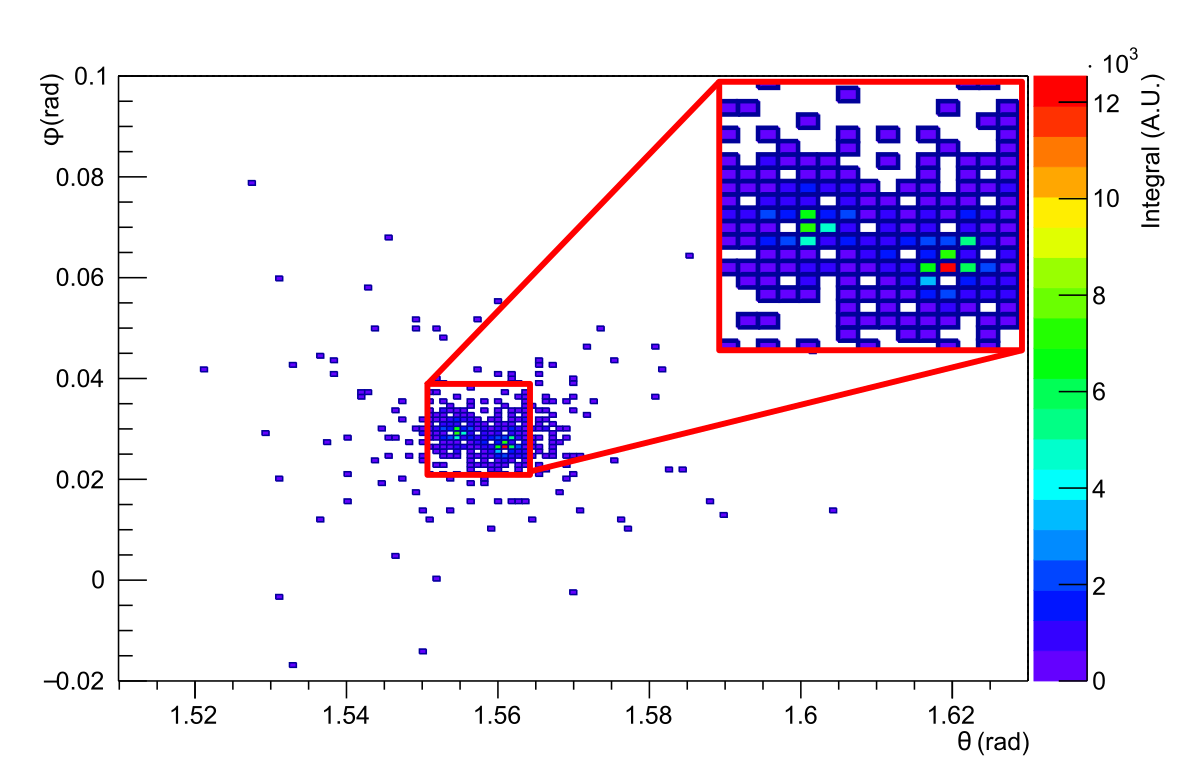
\includegraphics[width=.8\textwidth]{IMG/Cap6/Pizero40GeV_ev15_cher_hist_flat_zoom.png}} \quad
	\subfloat[][Scintillation signal post data setup.]{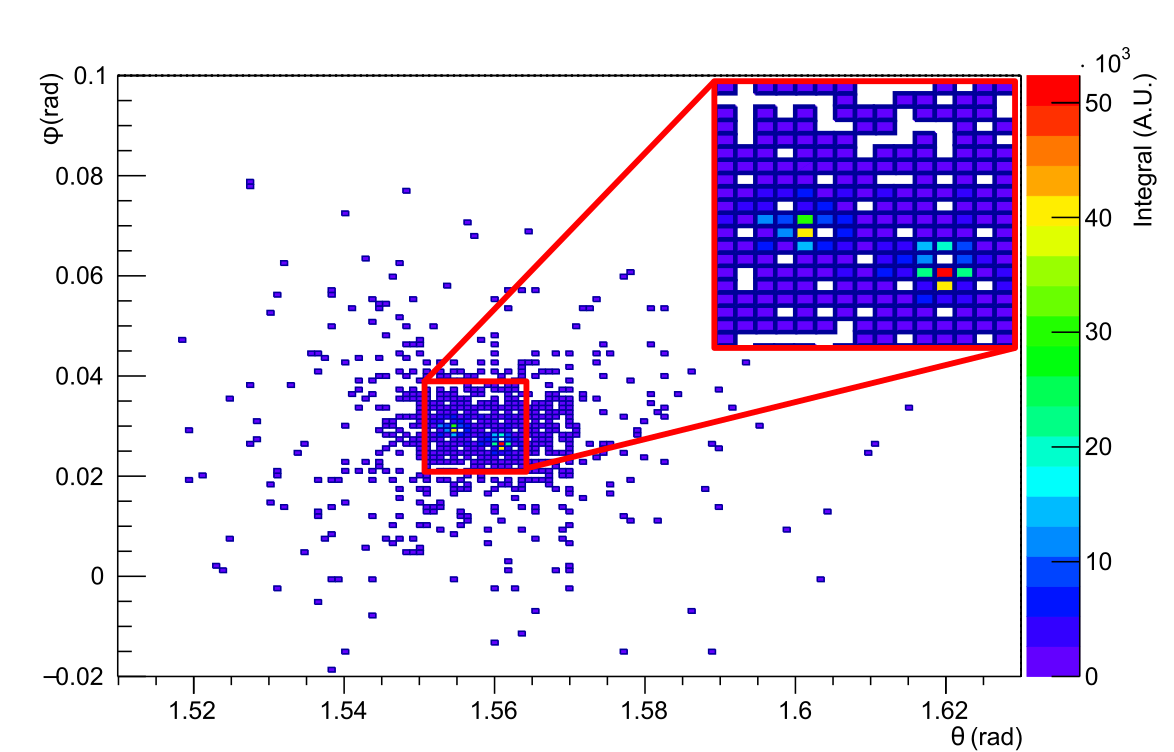
\includegraphics[width=.8\textwidth]{IMG/Cap6/Pizero40GeV_ev15_scin_hist_flat_zoom.png}}
	\caption{2D-vision of data after data preparation. Data from a $40$ GeV pion.}
	\label{fig:2Dvision4}
\end{figure}

The dataset is made of $10000$ events of photons and $10000$ events of neutral pions. All the events have been labelled ($\gamma$ or $\pi^0$), normalized to the max value of $1$, shuffled and splitted in two sub-set dedicated to training ($80\%$ of the whole statistics) and to validation ($20\%$ of the whole statistics).\\

\section{Performance}\label{sec:NN_perf}
Analyses of the performance of the two different convolutional neural network structures have been performed. Some of the \textit{hyperparameters} of the CNNs, namely all the parameters that identify the structure of the networks such as the number of layers, the number of filters and the kernel size in convolutional layers, the number of neurons in dense layers, have been modifyed to identify the optimal set of values.\\
This section shows the comparison between CNNs with different hyperparameters and details of the best performance obtained with the VGGNet and the ResNet.

\subsection{VGG Network}
The VGG neural networks used for the particle ID task follow the structure described in Section \ref{subsec:VGGNet_teo}.\\
The input and output are well defined by the data preparation and the classification task. The input is a 3D matrix with dimensions of $133 \times 133 \times 2$. The aim of distinguishing between two types of primary particle sets the output layer as a dense layer with two neurons, with Softmax as the activation function.\\
The optimisation process has to take into account a very large number of hyperparameters combinations; to make it simple and tidy, the layers can be divided in two groups separated by the flatten one: the "convolutional half" and the "dense half". The halves have been analysed one at a time by keeping fixed the other one and changing the hyperparameters within common value ranges.\\
In Table \ref{fig:VGGNet-tested}, the structures of the six different VGGNet tested are shown together with the accuracy value and the training time needed to evaluate the performance. The training process have been performed with $10$ threads at a clock speed of $5$ GHz.\\
The neural networks labelled as VGGNet A, VGGNet B and VGGNet C have the aim to optimize the dense half modifying the Dropout probability. Once the best dense half has been fixed VGGNet D, E and F have been tested to select the best hyperparameters in the convolution half. The conclusion from this study identifies VGGNet D as the best structure, with an accuracy of $98.875\%$ and a training time of $212$ s$/$epoch.\\

\begin{sidewaystable}
    \centering
    %\resizebox{\textwidth}{!}
    \tiny
    \begin{tabular}{l|l|l|l|l|l|l}
         \toprule
         &\textbf{VGGNet A} & \textbf{VGGNet B} & \textbf{VGGNet C} & \textbf{VGGNet D} & \textbf{VGGNet E} & \textbf{VGGNet F} \\
         \midrule
         
         &Input ($133\times133\times2$) & Input ($133\times133\times2$) & Input ($133\times133\times2$) & Input ($133\times133\times2$) & Input ($133\times133\times2$) & Input ($133\times133\times2$) \\
         
         &Conv2D ($32,3\times3$,ReLU) & Conv2D ($32,3\times3$,ReLU) & Conv2D ($32,3\times3$,ReLU) & Conv2D ($32,3\times3$,ReLU) & Conv2D ($32,3\times3$,ReLU) & Conv2D ($32,3\times3$,ReLU) \\
         
         &Conv2D ($32,3\times3$,ReLU) & Conv2D ($32,3\times3$,ReLU) & Conv2D ($23,3\times3$,ReLU) & Conv2D ($32,3\times3$,ReLU) & Conv2D ($32,3\times3$,ReLU) & Conv2D ($32,3\times3$,ReLU) \\
         
         &MaxPool (2x2) & MaxPool (2x2) & MaxPool (2x2) & MaxPool (2x2) & MaxPool (2x2) & MaxPool (2x2) \\
         \midrule
         
         &Conv2D ($64,3\times3$,ReLU) & Conv2D ($64,3\times3$,ReLU) & Conv2D ($64,3\times3$,ReLU) & Conv2D ($64,3\times3$,ReLU) & Conv2D ($32,3\times3$,ReLU) & Conv2D ($64,3\times3$,ReLU) \\
         
         &Conv2D ($64,3\times3$,ReLU) & Conv2D ($64,3\times3$,ReLU) & Conv2D ($64,3\times3$,ReLU) & Conv2D ($64,3\times3$,ReLU) & Conv2D ($32,3\times3$,ReLU) & Conv2D ($64,3\times3$,ReLU) \\
         
         &MaxPool (2x2) & MaxPool (2x2) & MaxPool (2x2) & MaxPool (2x2) & MaxPool (2x2) & MaxPool (2x2) \\
         \midrule
         
         &Conv2D ($128,3\times3$,ReLU) & Conv2D ($128,3\times3$,ReLU) & Conv2D ($128,3\times3$,ReLU) & Conv2D ($64,3\times3$,ReLU) & Conv2D ($64,3\times3$,ReLU) & Conv2D ($128,3\times3$,ReLU) \\
         
         &Conv2D ($128,3\times3$,ReLU) & Conv2D ($128,3\times3$,ReLU) & Conv2D ($128,3\times3$,ReLU) & Conv2D ($64,3\times3$,ReLU) & Conv2D ($64,3\times3$,ReLU) & Conv2D ($128,3\times3$,ReLU) \\
         
         &MaxPool (2x2) & MaxPool (2x2) & MaxPool (2x2) & MaxPool (2x2) & MaxPool (2x2) & MaxPool (2x2) \\
         \midrule
         
         &Conv2D ($128,3\times3$,ReLU) & Conv2D ($128,3\times3$,ReLU) & Conv2D ($128,3\times3$,ReLU) & Conv2D ($128,3\times3$,ReLU) & Conv2D ($64,3\times3$,ReLU) & Conv2D ($256,3\times3$,ReLU) \\
         
         &Conv2D ($128,3\times3$,ReLU) & Conv2D ($128,3\times3$,ReLU) & Conv2D ($128,3\times3$,ReLU) & Conv2D ($128,3\times3$,ReLU) & Conv2D ($64,3\times3$,ReLU) & Conv2D ($256,3\times3$,ReLU) \\
         
         &MaxPool (2x2) & MaxPool (2x2) & MaxPool (2x2) & MaxPool (2x2) & MaxPool (2x2) & MaxPool (2x2) \\
         \midrule         
         
         &Conv2D ($128,3\times3$,ReLU) & Conv2D ($128,3\times3$,ReLU) & Conv2D ($128,3\times3$,ReLU) & Conv2D ($128,3\times3$,ReLU) & Conv2D ($64,3\times3$,ReLU) & Conv2D ($256,3\times3$,ReLU) \\
         
         &Conv2D ($128,3\times3$,ReLU) & Conv2D ($128,3\times3$,ReLU) & Conv2D ($128,3\times3$,ReLU) & Conv2D ($128,3\times3$,ReLU) & Conv2D ($64,3\times3$,ReLU) & Conv2D ($256,3\times3$,ReLU) \\
         
         &MaxPool (2x2) & MaxPool (2x2) & MaxPool (2x2) & MaxPool (2x2) & MaxPool (2x2) & MaxPool (2x2) \\
         \midrule          
         
         &Flatten & Flatten & Flatten & Flatten & Flatten & Flatten \\
         
         &Dense(256,ReLU) & Dense(256,ReLU) & Dense(256,ReLU) & Dense(256,ReLU) & Dense(256,ReLU) & Dense(256,ReLU) \\
         
          & Dropout(0.3) & Dropout(0.5) & Dropout(0.5) & Dropout(0.5) & Dropout(0.5) \\
         
         &Dense(256,ReLU) & Dense(256,ReLU) & Dense(256,ReLU) & Dense(256,ReLU) & Dense(256,ReLU) & Dense(256,ReLU) \\
         
          & Dropout(0.3) & Dropout(0.5) & Dropout(0.5) & Dropout(0.5) & Dropout(0.5) \\
         
         &Output(2,SoftMax) & Output(2,SoftMax) & Output(2,SoftMax) & Output(2,SoftMax) & Output(2,SoftMax) & Output(2,SoftMax) \\
         \midrule
         Acc. & $97.275\%$ & $97.650\%$ & $97.660\%$ & $98.875\%$ & $97.299\%$ & $97.450\%$ \\
         Time &  $230$ s$/$epoch & $229$ s$/$epoch & $228$ s$/$epoch & $212$ s$/$epoch & $170$ s$/$epoch & $240$ s$/$epoch\\
         \bottomrule
    \end{tabular}
    \caption{Table listing the different VGGNet structures studied. Performance is evaluated by looking at the accuracy and the training time.}
    \label{fig:VGGNet-tested}
\end{sidewaystable}

Further studies on the performance have been done using VGGNet D.
The training was done with a training dataset and validated at each epoch on a validation dataset.
The accuracy was evaluated as the number of correct predictions over the total number of predictions ($n_c/N$). Figure \ref{fig:VGGNet-acc} shows the behaviour of the accuracy during the training process and compares the results for the training and the validation datasets.\\

\begin{figure}
	\centering
	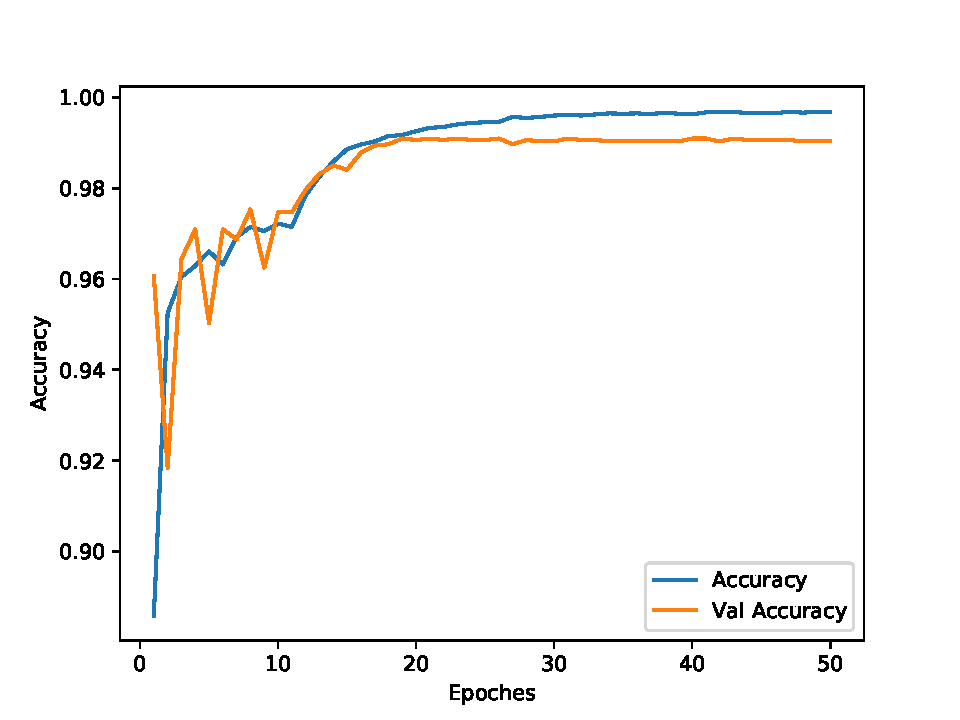
\includegraphics[width=0.85\textwidth]{IMG/Cap6/VGGNet-D_Accuracy.pdf}
	\caption{Accuracy behaviour over $50$ training epoches using the selected VGGNet. Train and validation accuracy are shown with different colours. Results for a $40$ GeV $\pi^0/\gamma$ events simulated with the IDEA calorimeter simulation chain.}
	\label{fig:VGGNet-acc}
\end{figure}

The loss function is another important feature that can be studied. It has been already introduced as the error function \ref{eq:err_func}. A loss value can be evaluated at the end of each training epoch to monitor the improvements in each training step. Figure \ref{fig:VGGNet-loss} shows its behaviour as a function of the training epoches.\\

\begin{figure}
	\centering
	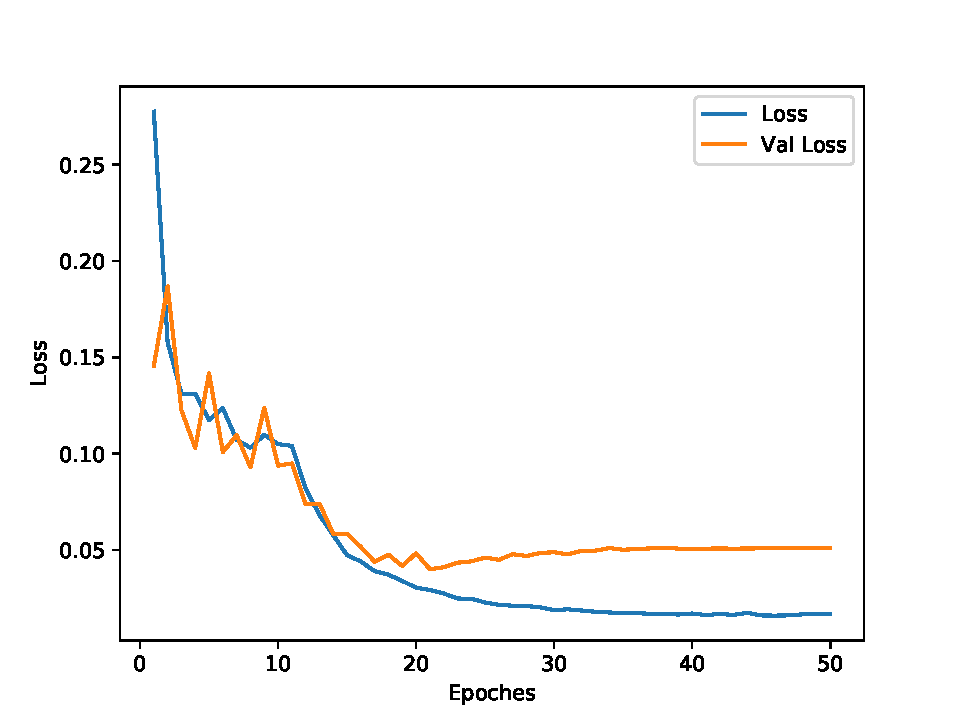
\includegraphics[width=0.85\textwidth]{IMG/Cap6/VGGNet-D_Loss.pdf}
	\caption{Loss behaviour over $50$ training epoches using the selected VGGNet. Train and validation losses are shown with different colors. Results for a $40$ GeV $\pi^0/\gamma$ events simulated with the IDEA calorimeter simulation chain.}
	\label{fig:VGGNet-loss}
\end{figure}

The smoothness of both accuracy and loss plots is an indication of the good dataset size; the graphs would typically show spikes, if a too small dataset were used. \\

Results on classification problems are often represented in confusion matrices, matrices showing the percentage probability of a neural network in identifying categories emphasizing true positive, true negative, false positive and false negative. The confusion matrix obtained with the selected VGGNet (trained for $50$ epoches) is shown in Figure \ref{fig:VGGNet-cm}.

\begin{figure}
	\centering
	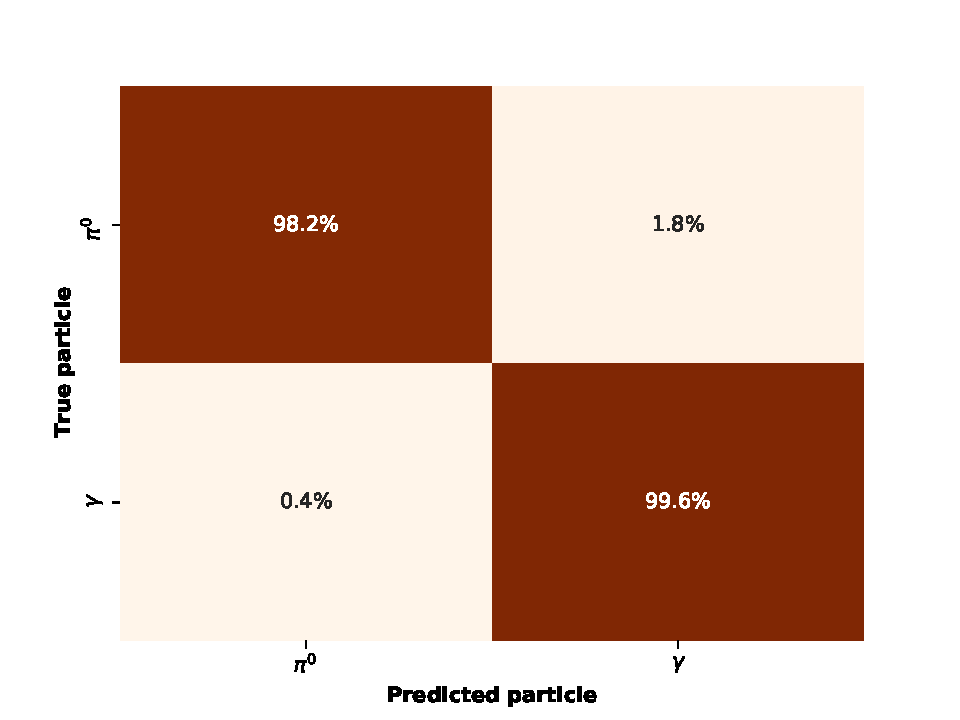
\includegraphics[width=0.85\textwidth]{IMG/Cap6/VGGNet-D_ConfMatrix.pdf}
	\caption{Confusion matrix obtained with test data using the selected VGGNet. Values are normalized on rows (i.e. on the true label). Results for a $40$ GeV $\pi^0/\gamma$ events simulated with the IDEA calorimeter simulation chain.}
	\label{fig:VGGNet-cm}
\end{figure}

\subsection{Residual Network}
The residual neural networks used for the particle ID task follows the structure described in Section \ref{subsec:ResNet_teo}.\\
The input and output of the ResNets has to coincide with the ones for VGGNets, due to the same data preparation process and the same classification task. The input data will have a 3D matrix shape ($133\times 133\times 2$) and the last layer is set to be a two-neurons dense layer with the Softmax activation function, corresponding to the probability of identifying a photon or a neutral pion.\\
%The articulation of the middle layers follows the typical ResNet structure presented in Section \ref{subsec:ResNet_teo}.\\
As done for the VGGNet optimization, also this structure has been divided in two parts identified by the \textit{GlobalAveragePooling} layer ("convolutional half" and "dense half"). In Table \ref{fig:ResNet-tested} the six different ResNet with different hyperparameters are listed. ResNet A, B, C and D are dedicated to the optimisation of the dense half. Once the best dense half structure has been found, the ResNet E and F have been trained to find the best ResNet for the convolutional task. As schematically shown in the table, ResNet D has the best performances with an accuracy of $97.275\%$ and a training time of $192$ s$/$epoch.\\

\begin{sidewaystable}
    \centering
    %\resizebox{\textwidth}{!}
    \tiny
    \begin{tabular}{l|l|l|l|l|l|l}
         \toprule
         &\textbf{ResNet A} & \textbf{ResNet B} & \textbf{ResNet C} & \textbf{ResNet D} & \textbf{ResNet E} & \textbf{ResNet F} \\
         \midrule
         
         &Input ($133\times133\times2$) & Input ($133\times133\times2$) & Input ($133\times133\times2$) & Input ($133\times133\times2$) & Input ($133\times133\times2$) & Input ($133\times133\times2$) \\
         
         &Conv2D ($64,3\times3$,ReLU) & Conv2D ($64,3\times3$,ReLU) & Conv2D ($64,3\times3$,ReLU) & Conv2D ($64,3\times3$,ReLU) & Conv2D ($32,3\times3$,ReLU) & Conv2D ($64,3\times3$,ReLU) \\
         
         &Conv2D ($64,3\times3$,ReLU) & Conv2D ($64,3\times3$,ReLU) & Conv2D ($64,3\times3$,ReLU) & Conv2D ($64,3\times3$,ReLU) & Conv2D ($32,3\times3$,ReLU) & Conv2D ($64,3\times3$,ReLU) \\
         \midrule
         
         &Conv2D ($64,3\times3$,ReLU) & Conv2D ($64,3\times3$,ReLU) & Conv2D ($64,3\times3$,ReLU) & Conv2D ($64,3\times3$,ReLU) & Conv2D ($32,3\times3$,ReLU) & Conv2D ($64,3\times3$,ReLU) \\
         
         &Conv2D ($64,3\times3$,ReLU) & Conv2D ($64,3\times3$,ReLU) & Conv2D ($64,3\times3$,ReLU) & Conv2D ($64,3\times3$,ReLU) & Conv2D ($32,3\times3$,ReLU) & Conv2D ($64,3\times3$,ReLU) \\
         
         & &  &  &  & Conv2D ($32,3\times3$,ReLU) & Conv2D ($64,3\times3$,ReLU) \\
         \midrule
         
         &Conv2D ($64,3\times3$,ReLU) & Conv2D ($64,3\times3$,ReLU) & Conv2D ($64,3\times3$,ReLU) & Conv2D ($64,3\times3$,ReLU) & Conv2D ($32,3\times3$,ReLU) & Conv2D ($64,3\times3$,ReLU) \\
         
         &Conv2D ($64,3\times3$,ReLU) & Conv2D ($64,3\times3$,ReLU) & Conv2D ($64,3\times3$,ReLU) & Conv2D ($64,3\times3$,ReLU) & Conv2D ($32,3\times3$,ReLU) & Conv2D ($64,3\times3$,ReLU) \\
         
         & &  &  &  & Conv2D ($32,3\times3$,ReLU) & Conv2D ($64,3\times3$,ReLU) \\
         \midrule
         
         &Conv2D ($64,3\times3$,ReLU) & Conv2D ($64,3\times3$,ReLU) & Conv2D ($64,3\times3$,ReLU) & Conv2D ($64,3\times3$,ReLU) & Conv2D ($32,3\times3$,ReLU) & Conv2D ($64,3\times3$,ReLU) \\
         
         &Conv2D ($64,3\times3$,ReLU) & Conv2D ($64,3\times3$,ReLU) & Conv2D ($64,3\times3$,ReLU) & Conv2D ($64,3\times3$,ReLU) & Conv2D ($32,3\times3$,ReLU) & Conv2D ($64,3\times3$,ReLU) \\
         
         & &  &  &  & Conv2D ($32,3\times3$,ReLU) & Conv2D ($64,3\times3$,ReLU) \\
         \midrule         
         
         &GlobalAveragePooling & GlobalAveragePooling & GlobalAveragePooling & GlobalAveragePooling & GlobalAveragePooling & GlobalAveragePooling \\
         
         &Dense(256,ReLU) & Dense(256,ReLU) & Dense(256,ReLU) & Dense(128,ReLU) & Dense(128,ReLU) & Dense(128,ReLU) \\
         
         & & Dropout(0.3) & Dropout(0.5) & Dropout(0.5) & Dropout(0.5) & Dropout(0.5) \\
         
         &Dense(256,ReLU) & Dense(256,ReLU) & Dense(256,ReLU) & Dense(128,ReLU) & Dense(128,ReLU) & Dense(128,ReLU) \\
         
         & & Dropout(0.3) & Dropout(0.5) & Dropout(0.5) & Dropout(0.5) & Dropout(0.5) \\
         
         &Output(2,SoftMax) & Output(2,SoftMax) & Output(2,SoftMax) & Output(2,SoftMax) & Output(2,SoftMax) & Output(2,SoftMax) \\
         \midrule
         Acc. & $96.875\%$ & $96.700\%$ & $96.525\%$ & $97.275\%$ & $96.850\%$ & $97.000\%$ \\
         Time & $223$ s$/$epoch &  $207$ s$/$epoch & $198$ s$/$epoch & $192$ s$/$epoch & $183$ s$/$epoch & $389$ s$/$epoch\\
         \bottomrule
    \end{tabular}
    \caption{Table of different ResNet structure studied. The performance is evaluated by looking at the accuracy and training time values. Note that the thicker lines divide the different Recurrent blocks as described in Section \ref{subsec:ResNet_teo}.}
    \label{fig:ResNet-tested}
\end{sidewaystable}

The Residual Network performance, as the VGG Network one, has been studied under the same conditions such as batch size ($128$ events) and number of training epoches ($50$), using also the same accuracy and loss evaluation functions.\\
Both accuracy and loss values have been recorded during the training process and their behaviour with respect to the training epoches is shown in Figures \ref{fig:ResNet-acc} and \ref{fig:ResNet-loss}.

\begin{figure}
	\centering
	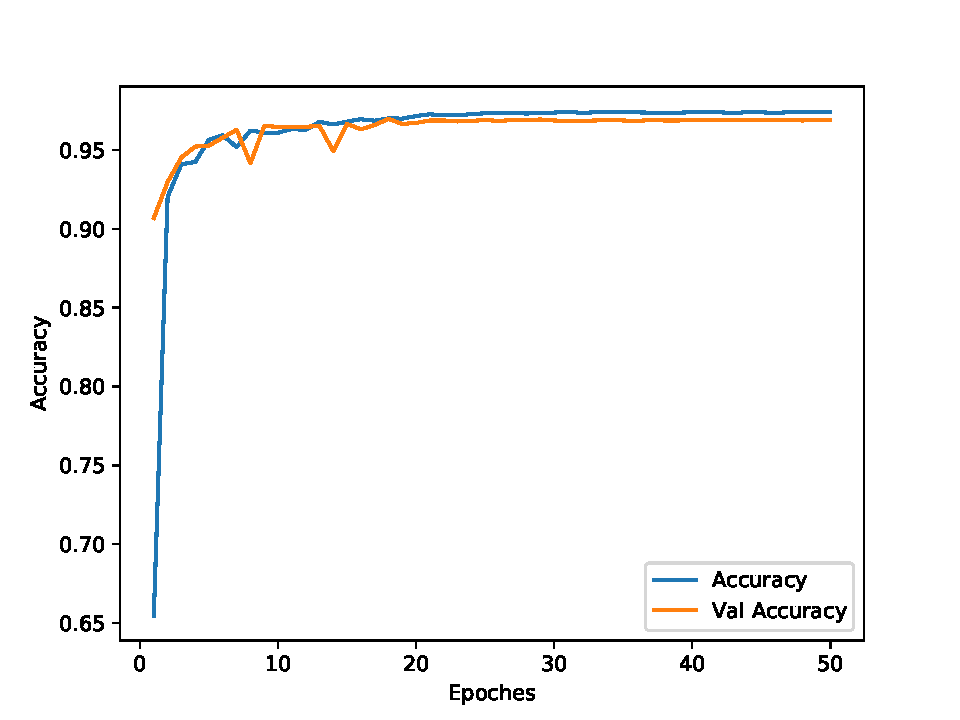
\includegraphics[width=0.85\textwidth]{IMG/Cap6/ResNet-D_Accuracy.pdf}
	\caption{Accuracy behaviour over $50$ training epoches using the selected ResNet. Train and validation accuracy are shown with different colours. Results for a $40$ GeV $\pi^0/\gamma$ events simulated with the IDEA calorimeter simulation chain.}
	\label{fig:ResNet-acc}
\end{figure}

\begin{figure}
	\centering
	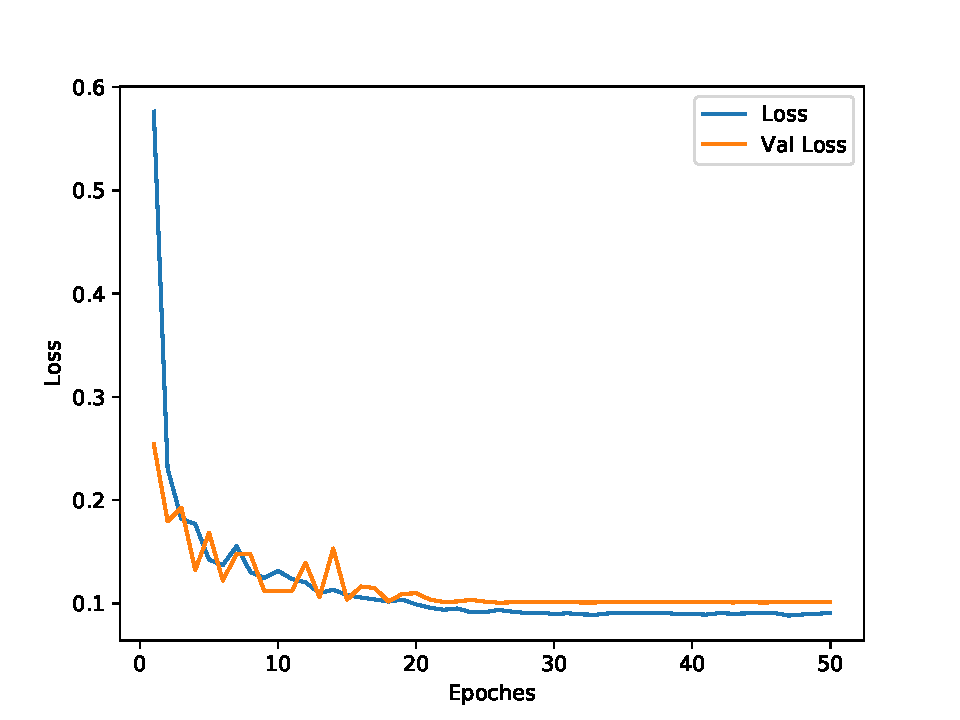
\includegraphics[width=0.85\textwidth]{IMG/Cap6/ResNet-D_Loss.pdf}
	\caption{Loss behaviour over $50$ training epoches using the selected ResNet. Train and validation loss are shown with different colours.  Results for a $40$ GeV $\pi^0/\gamma$ events simulated with the IDEA calorimeter simulation chain.}
	\label{fig:ResNet-loss}
\end{figure}

Also in this case a confusion matrix has been produced on validation data reaching the results shown in Figure \ref{fig:ResNet-cm}.

\begin{figure}
	\centering
	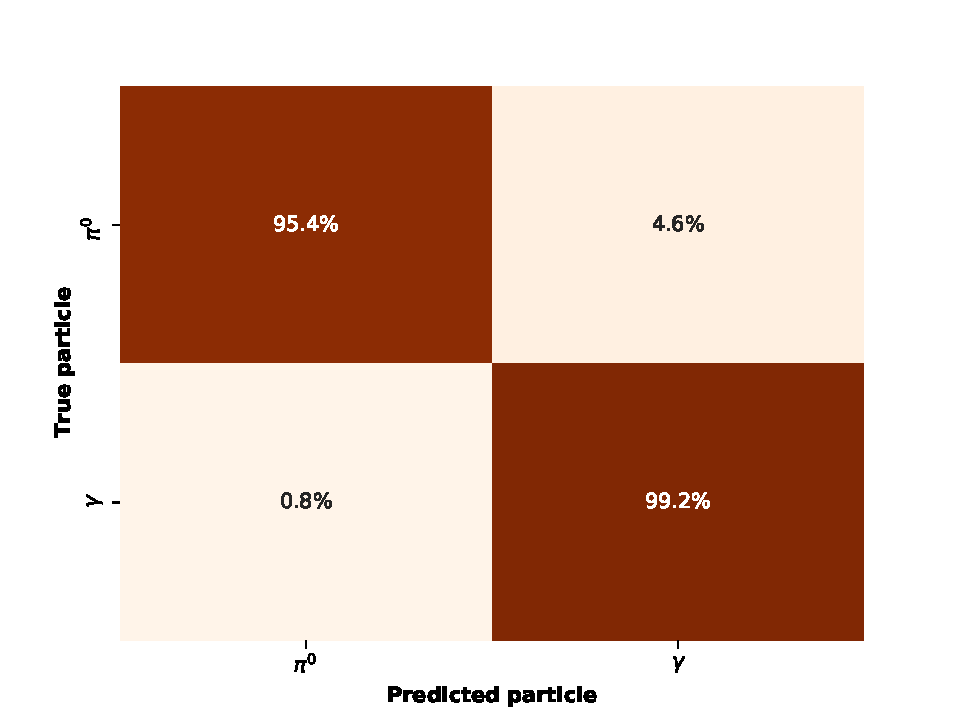
\includegraphics[width=0.85\textwidth]{IMG/Cap6/ResNet-D_ConfMatrix.pdf}
	\caption{Confusion matrix obtained with test data  using the selected ResNet. Values are normalized on rows (i.e. on the true label). Results for $40$ GeV $\pi^0/\gamma$ events simulated with the IDEA calorimeter simulation chain.}
	\label{fig:ResNet-cm}
\end{figure}

\section{Energy range extension}
Once the NN performances have been studied in the simplified case of photons and pions of $40$ GeV energy, the best structures (i.e. VGGNet D and ResNet D) have also been used to discriminate $\pi^0$ and $\gamma$ with energies ranging from $1$ to $80$ GeV.
This range will likely cover the one at future circular electroweak colliders where a particle, with unknown energy, interacts with the calorimeter and the neural network has to distinguish if the particle is a $\gamma$ or a superposition of $2\gamma$'s from a $\pi^0$ decay.
This task is only possible thanks to the high-granularity of the IDEA calorimeter. Standard today's calorimeters do not have the granularity required to perform this type of discrimination.\\

To perform this study, a set of $15000$ events for each particle type has been produced, in which the energy is uniformly distributed in the considered range. In this study we neglected the $\pi^0 \rightarrow e^+e^-\gamma$ process. 
The dataset production and preparation have been done following the same procedure previously described.\\
Once again the two neural networks have been trained over the $80\%$ of the data, reaching similar results in accuracy and loss performance (see Figures \ref{fig:VGGNet_acc_ERange}, \ref{fig:VGGNet_loss_ERange}, \ref{fig:ResNet_acc_ERange} and \ref{fig:ResNet_loss_ERange}). The validation process on the remaining $20\%$ of the dataset has provided the confusion matrices shown in Figure \ref{fig:CM_rangeE}.

\begin{figure}
	\centering
	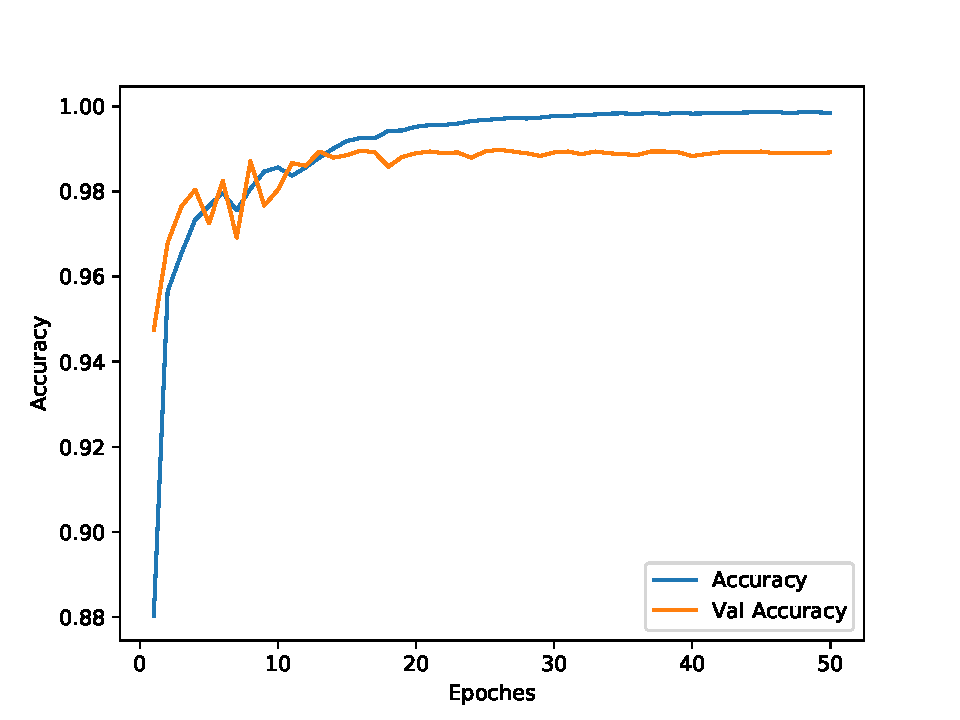
\includegraphics[width=0.85\textwidth]{IMG/Cap6/VGG_ERange_accuracy.pdf}
	\caption{Accuracy behaviour over $50$ training epoches using the selected VGGNet on events with variable energies. Train and validation accuracy are shown with different colours. Results for $1-80$ GeV $\pi^0/\gamma$ events simulated with the IDEA calorimeter simulation chain.}
	\label{fig:VGGNet_acc_ERange}
\end{figure}

\begin{figure}
	\centering
	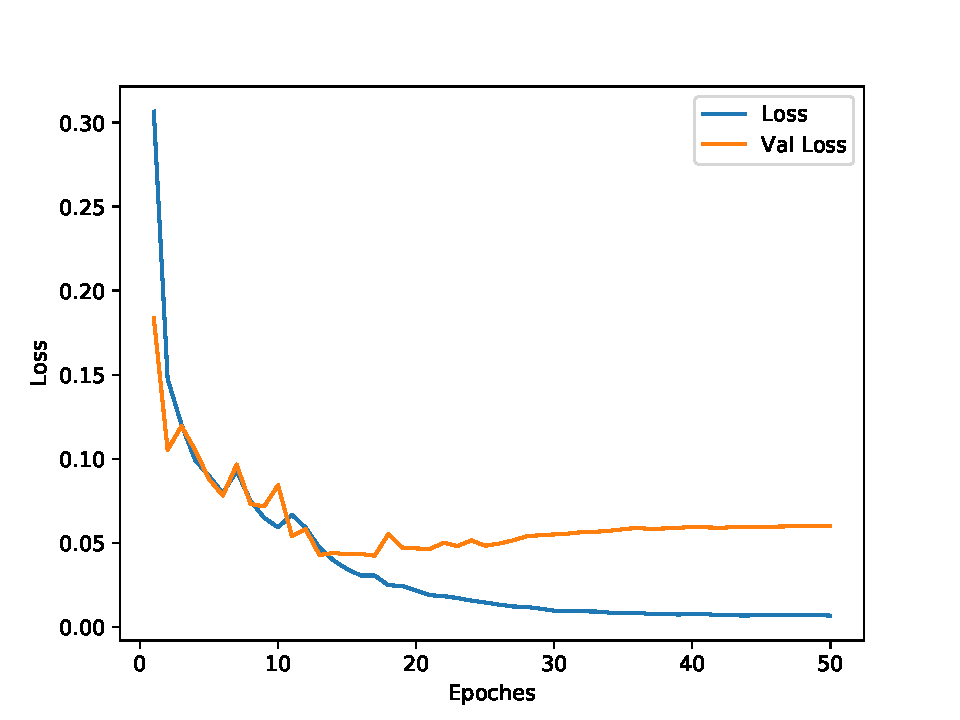
\includegraphics[width=0.85\textwidth]{IMG/Cap6/VGG_ERange_Loss.pdf}
	\caption{Loss behaviour over $50$ training epoches using the selected VGGNet on events with variable energies. Train and validation accuracy are shown with different colours. Results for $1-80$ GeV $\pi^0/\gamma$ events simulated with the IDEA calorimeter simulation chain.}
	\label{fig:VGGNet_loss_ERange}
\end{figure}

\begin{figure}
	\centering
	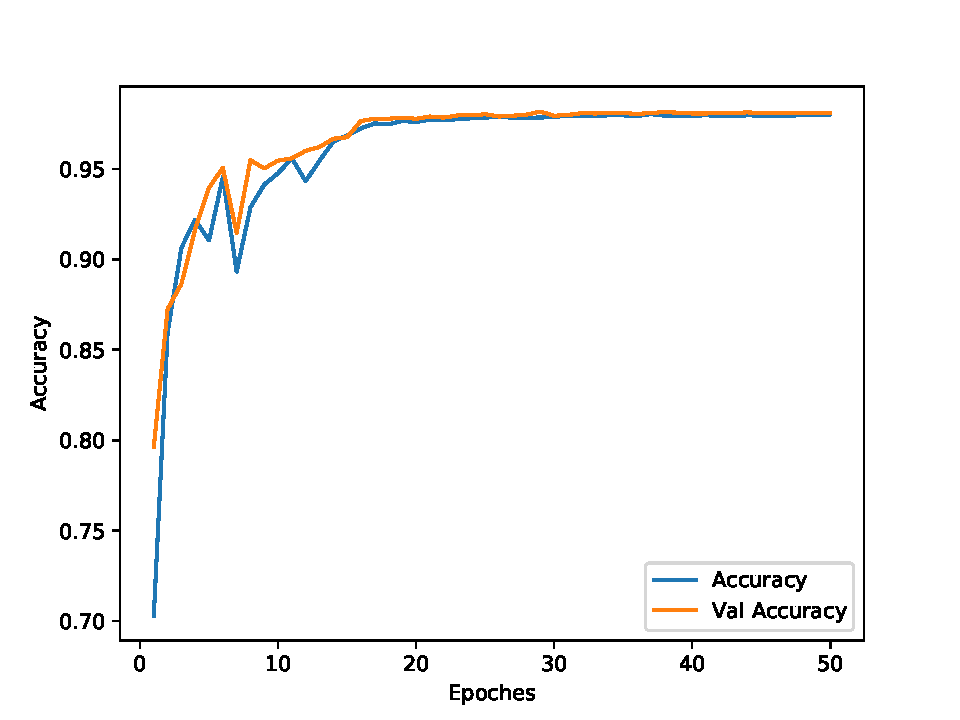
\includegraphics[width=0.85\textwidth]{IMG/Cap6/Res_ERange_accuracy.pdf}
	\caption{Accuracy behaviour over $50$ training epoches using the selected ResNet on events with variable energies. Train and validation accuracy are shown with different colours. Results for $1-80$ GeV $\pi^0/\gamma$ events simulated with the IDEA calorimeter simulation chain.}
	\label{fig:ResNet_acc_ERange}
\end{figure}

\begin{figure}
	\centering
	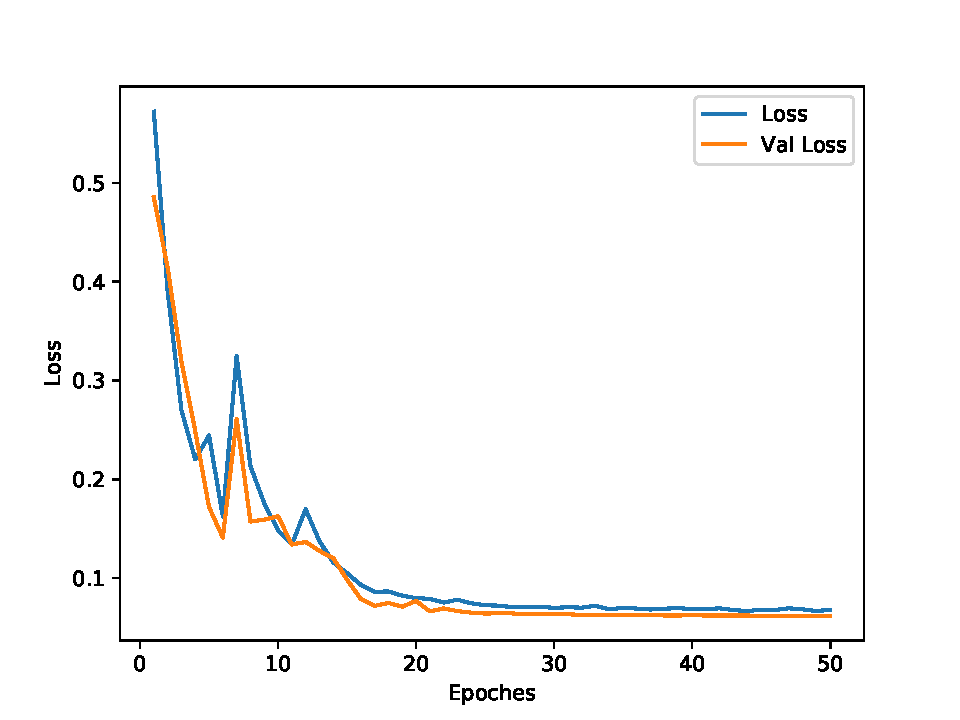
\includegraphics[width=0.85\textwidth]{IMG/Cap6/Res_ERange_Loss.pdf}
	\caption{Loss behaviour over $50$ training epoches using the selected ResNet on events with variable energies. Train and validation accuracy are shown with different colours. Results for $1-80$ GeV $\pi^0/\gamma$ events simulated with the IDEA calorimeter simulation chain.}
	\label{fig:ResNet_loss_ERange}
\end{figure}

\begin{figure}
	\centering
	\subfloat[][VGGNet structure.]{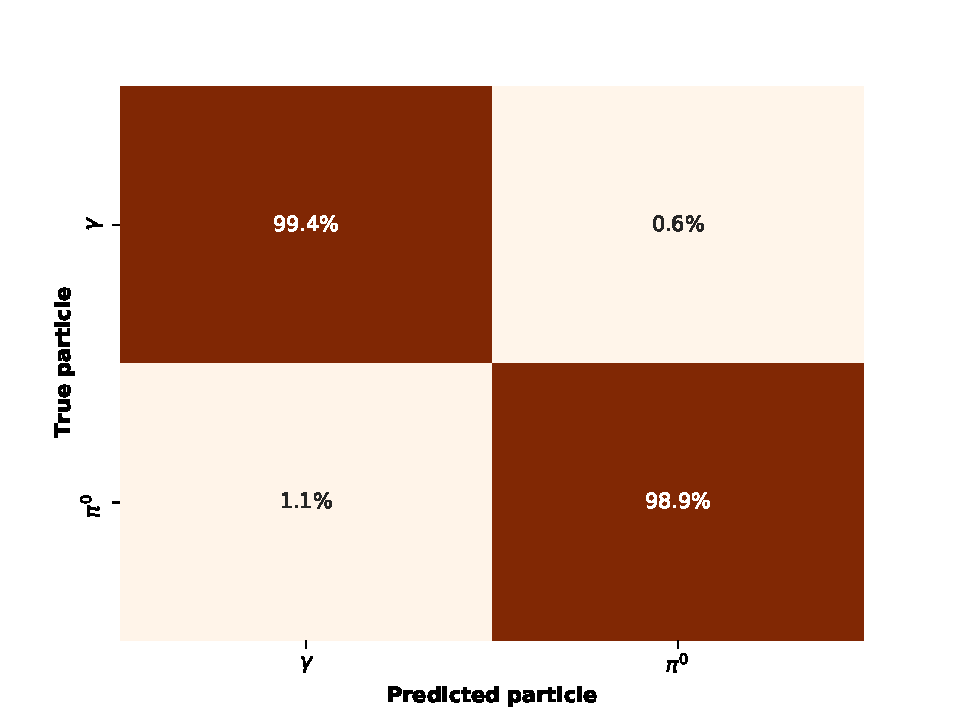
\includegraphics[width=.85\textwidth]{IMG/Cap6/VGG_ERange_ConfMatrix.pdf}} \quad
	\subfloat[][ResNet structure.]{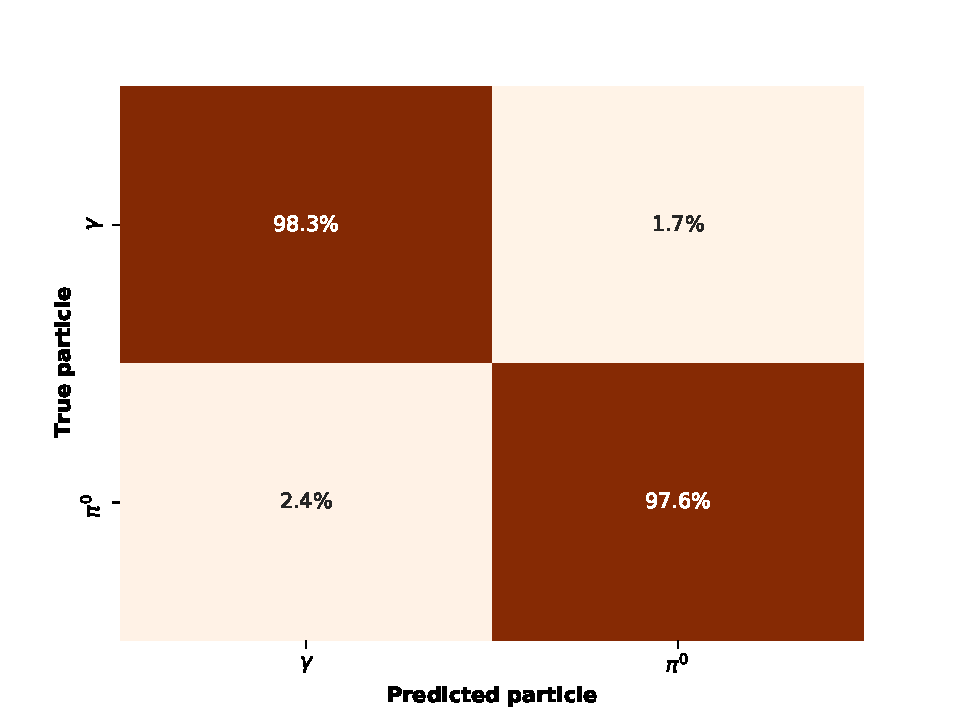
\includegraphics[width=.85\textwidth]{IMG/Cap6/Res_ERange_ConfMatrix.pdf}}
	\caption{The confusion matrices obtained in the validation process for data produced by $\gamma$ and $\pi^0$ with energies in the range $1 - 80$ GeV.}
	\label{fig:CM_rangeE}
\end{figure}

\subsection*{ROC and AUC}
A way to evaluate in more detail the correctness of a neural network in a classification task is the production of the Receiver Operating Characteristic curve (ROC curve) and the Area Under the ROC Curve (AUC).\\

Starting from the idea that the NN goal is to identify a neutral pion signal in a set of data where photon signals are also present, the focus has to be placed on the output neuron associated to the $\pi^0$.\\
A relevant plot, as the one shown in Figure \ref{fig:VGG_hist_pi} for the VGGNet, is the distribution of activation values associated to the neuron of interest, dividing them in two groups depending on the true particle producing the data.
In case of data from $\gamma$s, the closer to $0$ is the pion activation value, the more correct is the NN prediction.
On the other hand, in case of data from $\pi^0$s, the closer to $1$ is the pion activation value, the more correct is the NN prediction.\\
A neural network shows perfect classification capabilities when the two distribution are perfectly separated, one all below the $0.5$ activation value and the other one all above.\\

\begin{figure}
	\centering
	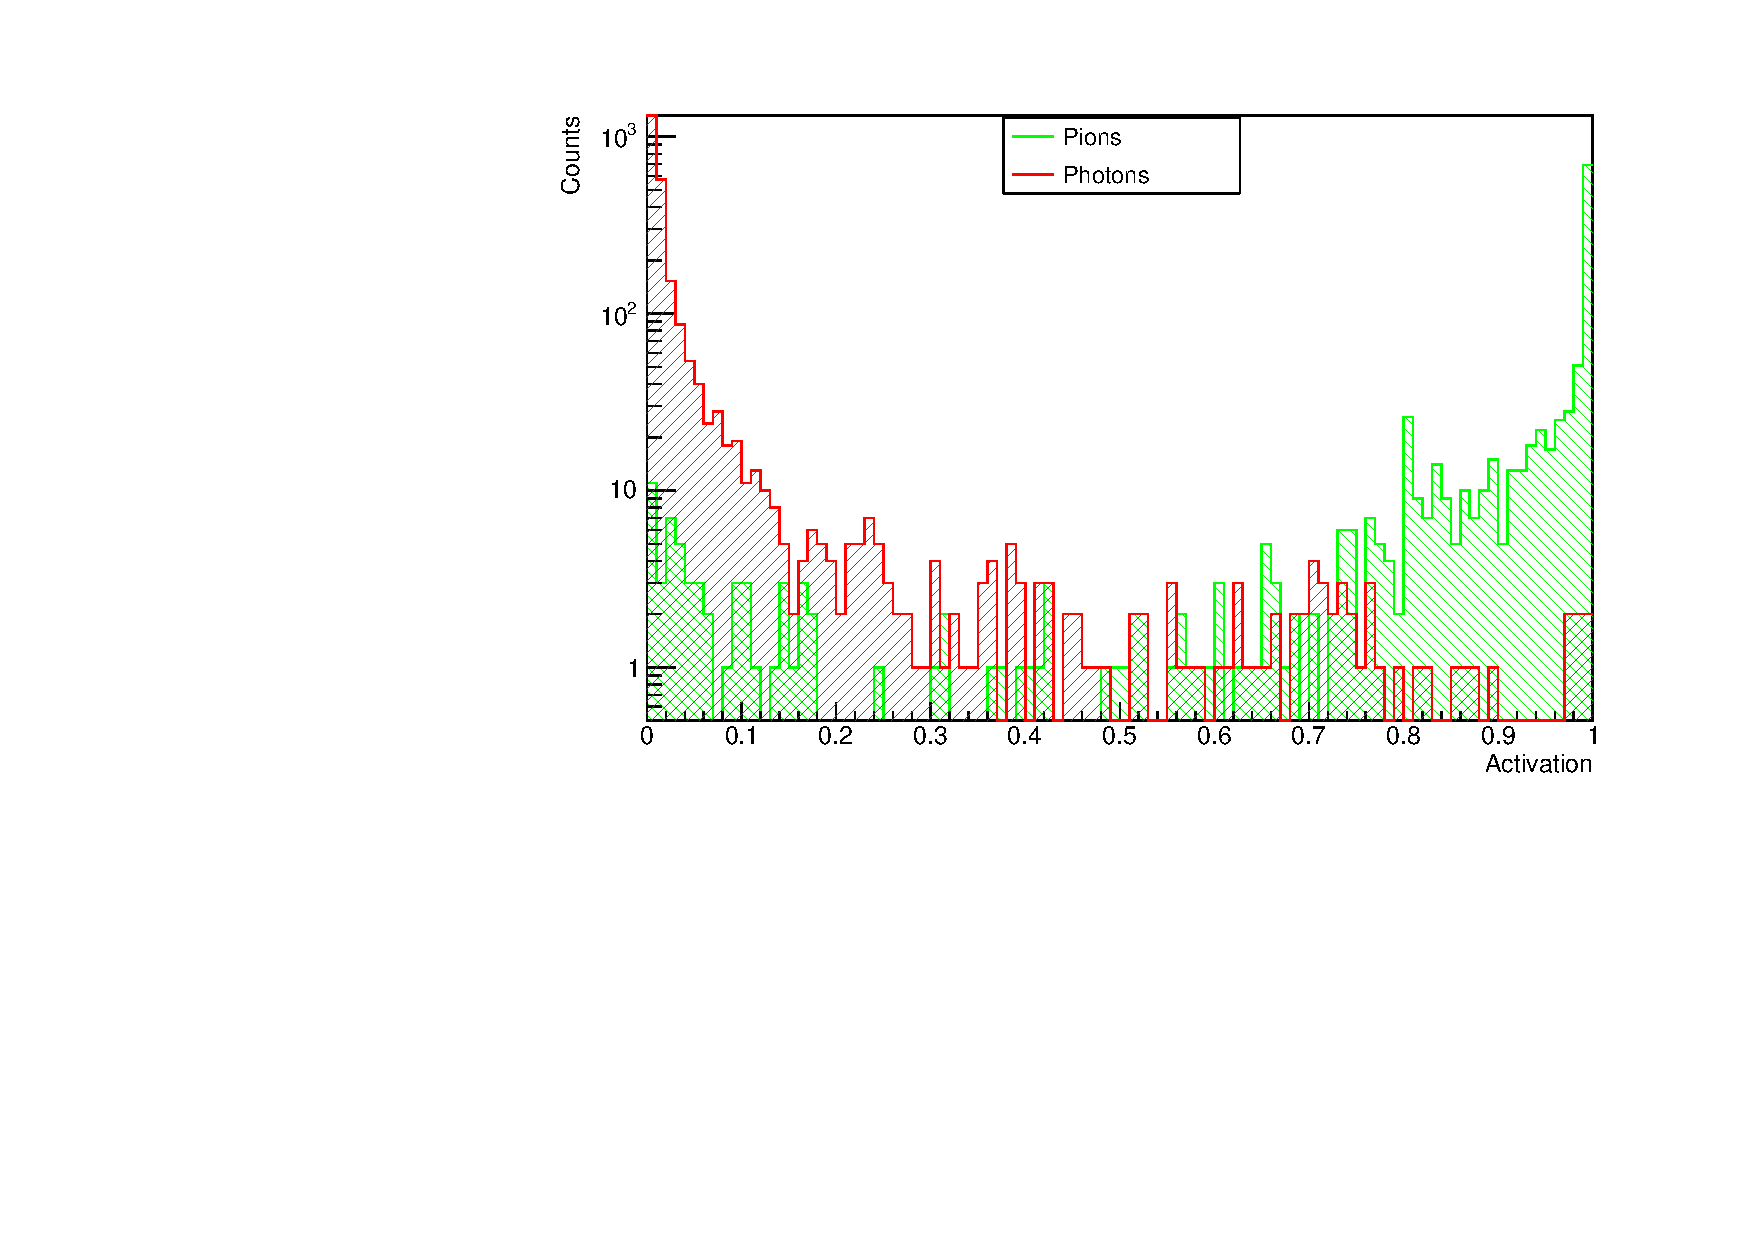
\includegraphics[width=0.85\textwidth]{IMG/Cap6/Res_hist_pi.pdf}
	\caption{Distributions of the $\pi^0$ neuron activation value for the VGGNet, divided in pion and photon events. Results for $1-80$ GeV $\pi^0/\gamma$ events simulated with the IDEA calorimeter simulation chain.}
	\label{fig:VGG_hist_pi}
\end{figure}

In 2-classes classification tasks, the threshold to consider a neuron activated is set at $0.5$ as default. Changing this value, different confusion matrices are produced, and the ROC curve is a practical way to summarise these matrices by changing the threshold. The ROC curve is obtained by plotting a point for each threshold value assigning as $x$ coordinate the efficiency in detecting a pion (i.e. the fraction of neutral pions correctly recognised) and as $y$ coordinate the rejection of photon events (i.e. the fraction of photons that are recognised as photons).\\
The ideal ROC curve is the one passing on the point $(1,1)$ that corresponds to the perfect efficiency and rejection conditions.\\
The area under this curve is called AUC and represents a numerical value that easily allows to compare different NN or conditions (the ideal AUC value is $1$).\\

The ROC curves obtained from the selected VGGNet and ResNet are shown in Figure \ref{fig:ROC} and the AUC values are $0.9982$ and $0.9957$ respectively.\\

ROC curves are also produced by dividing the validation dataset in sub-samples depending on the energies.
As the graphs \ref{fig:ROC_VGG_sub} and \ref{fig:ROC_Res_sub} show, in the range $1-80$ GeV the performance of the two neural networks are almost energy independent.

\begin{figure}
	\centering
	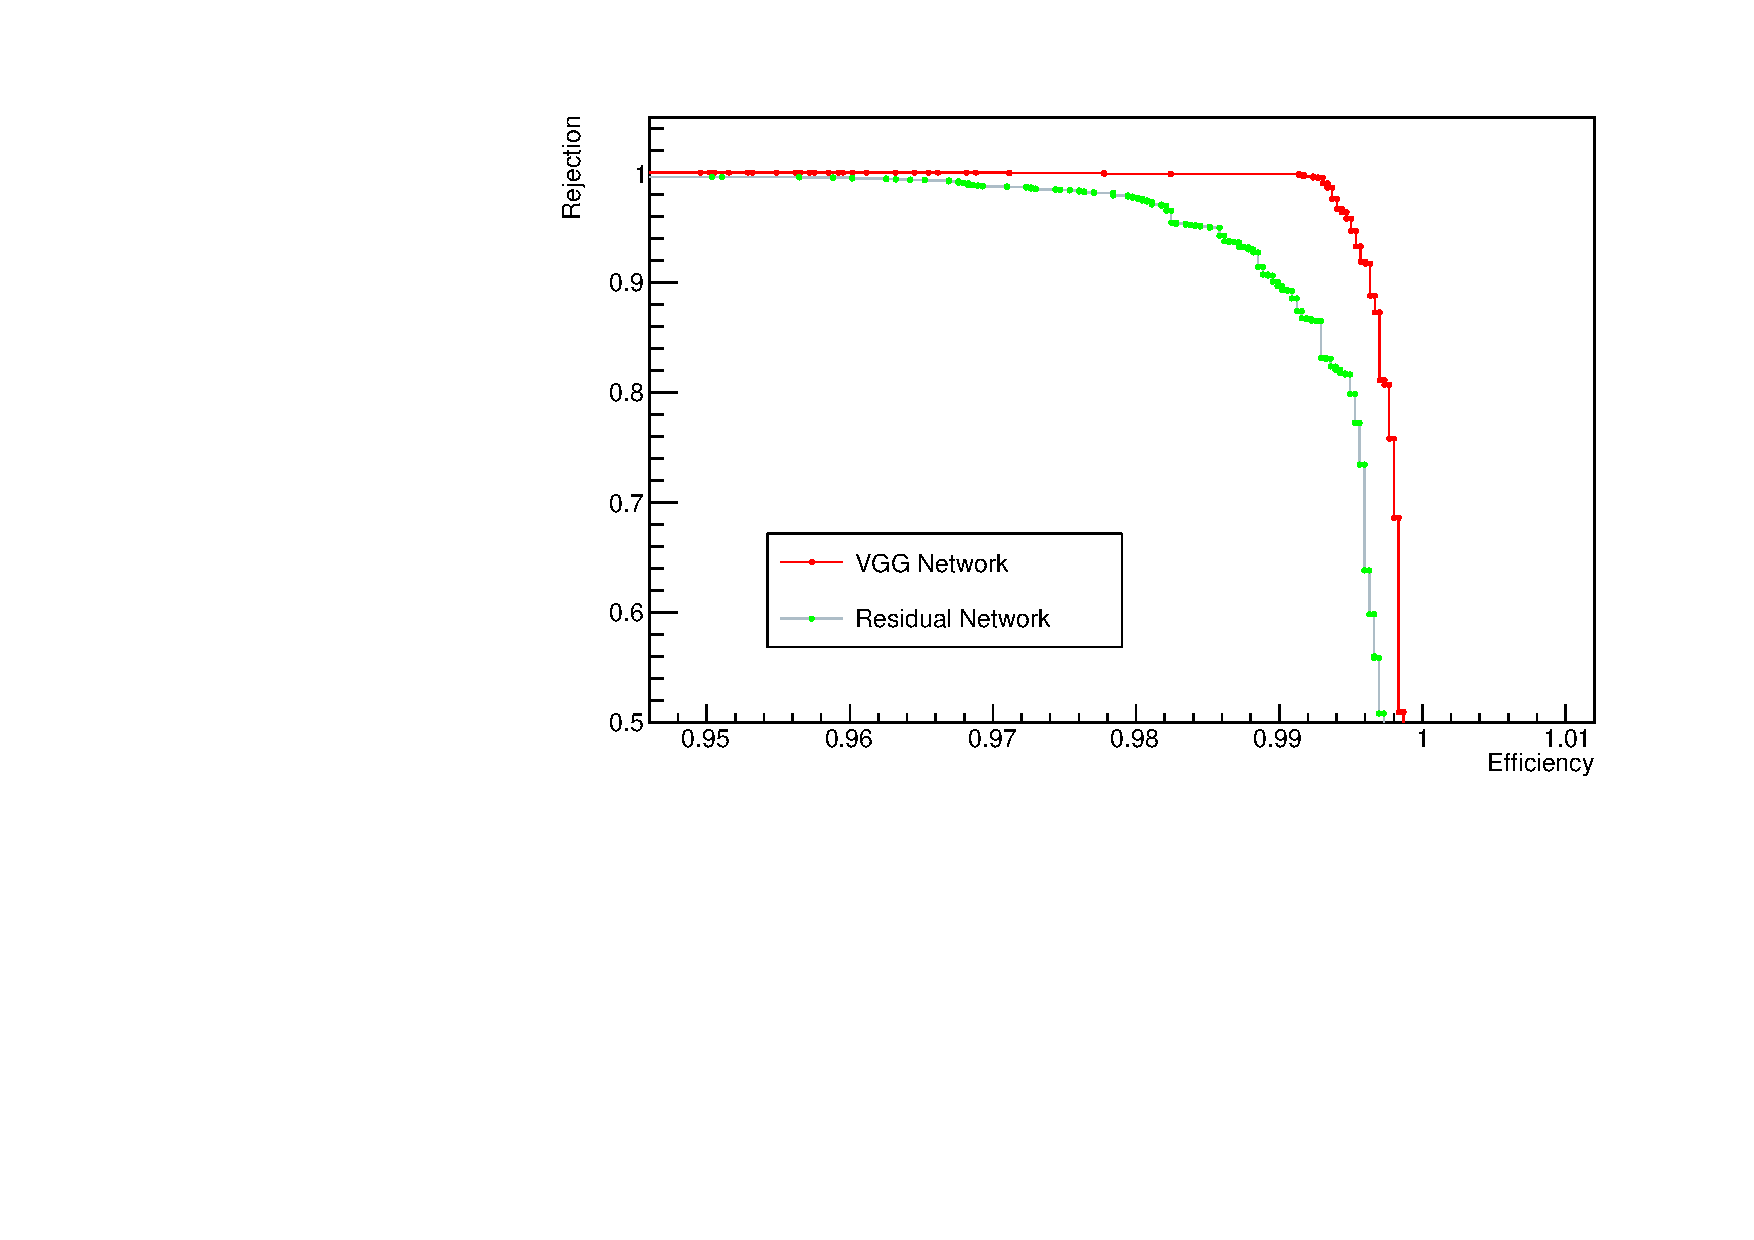
\includegraphics[width=0.85\textwidth]{IMG/Cap6/ROC_VGG_Res_zoom.pdf}
	\caption{ROC curve comparison for the two neural networks. Results for $1-80$ GeV $\pi^0/\gamma$ events simulated with the IDEA calorimeter simulation chain.}
	\label{fig:ROC}
\end{figure}

\begin{figure}
	\centering
	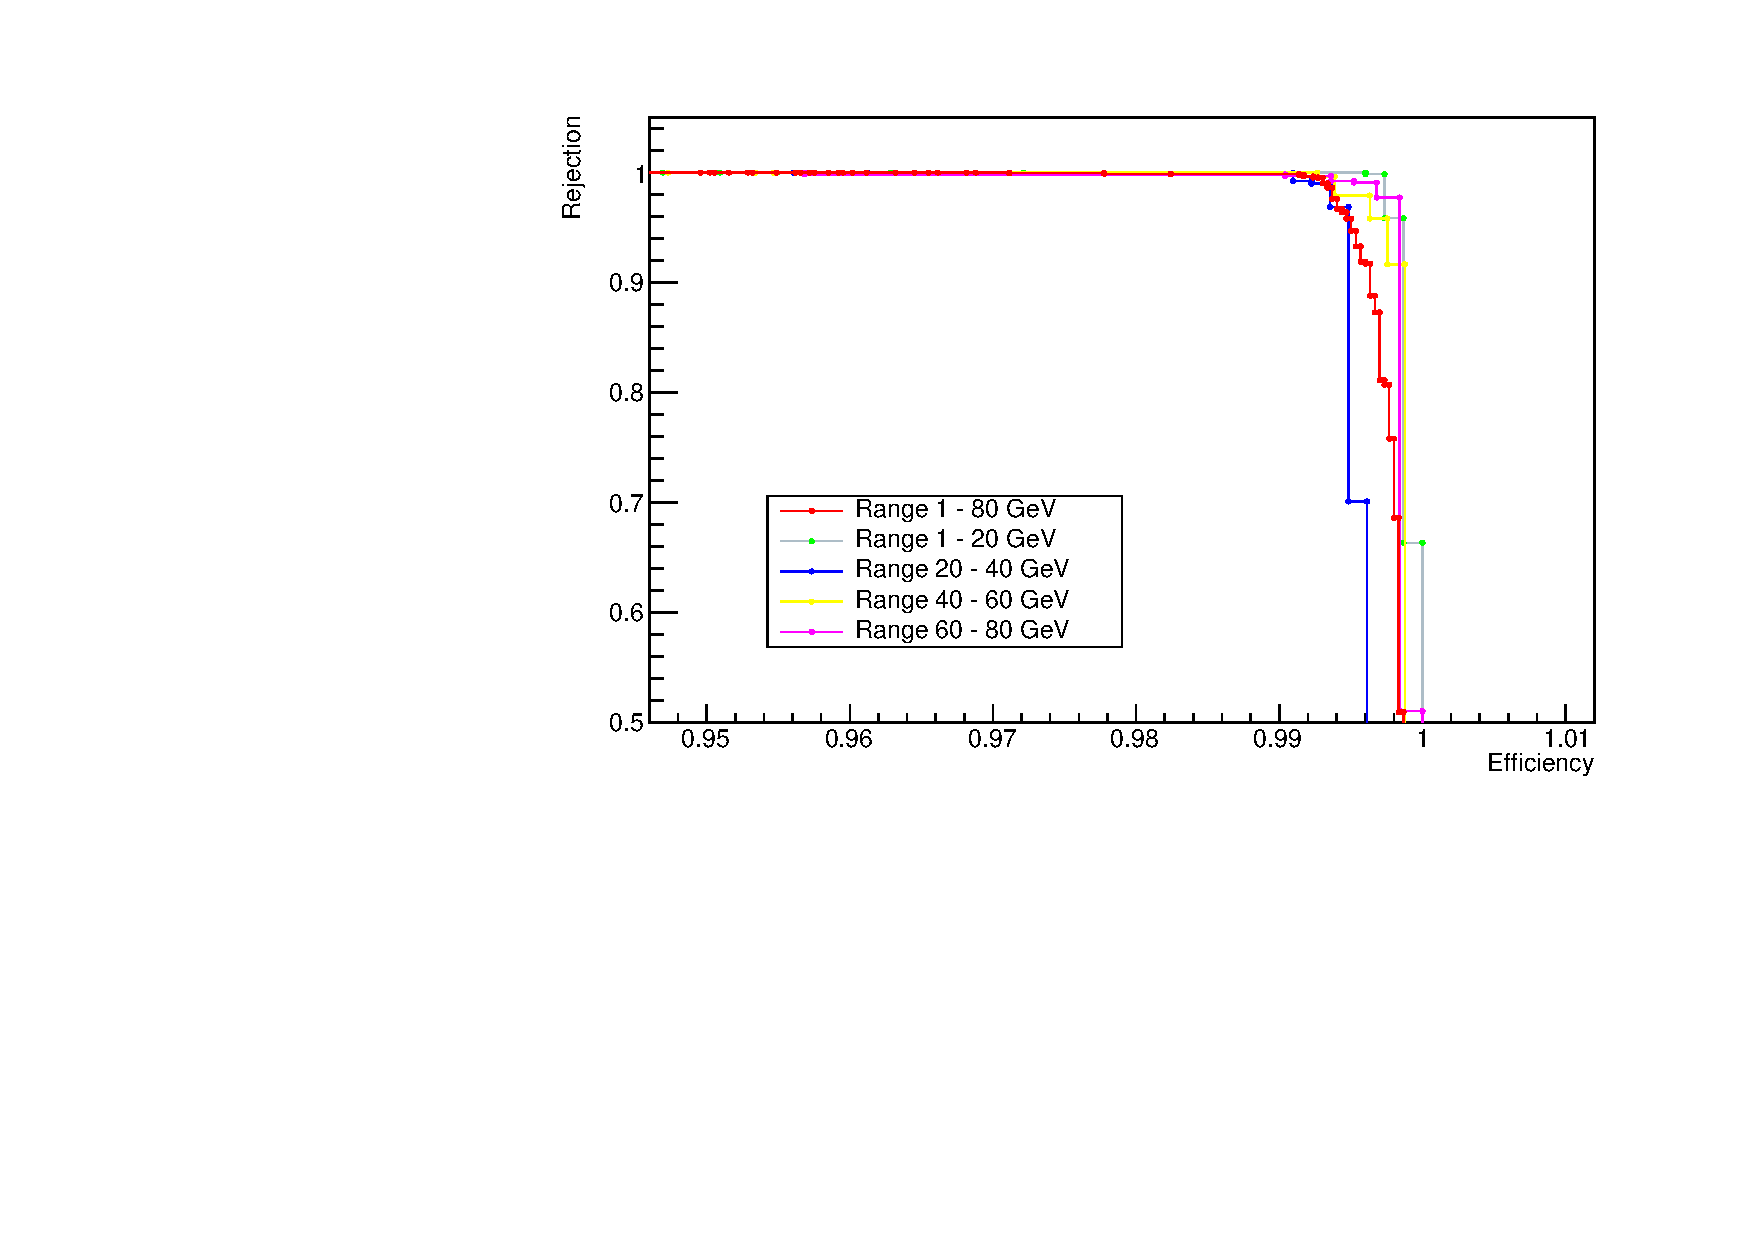
\includegraphics[width=0.85\textwidth]{IMG/Cap6/ROC_VGG_sub_zoom.pdf}
	\caption{ROC curves for the selected VGG Network over subsamples of events with different energies, as described in the legend. Results for $1-80$ GeV $\pi^0/\gamma$ events simulated with the IDEA calorimeter simulation chain.}
	\label{fig:ROC_VGG_sub}
\end{figure}

\begin{figure}
	\centering
	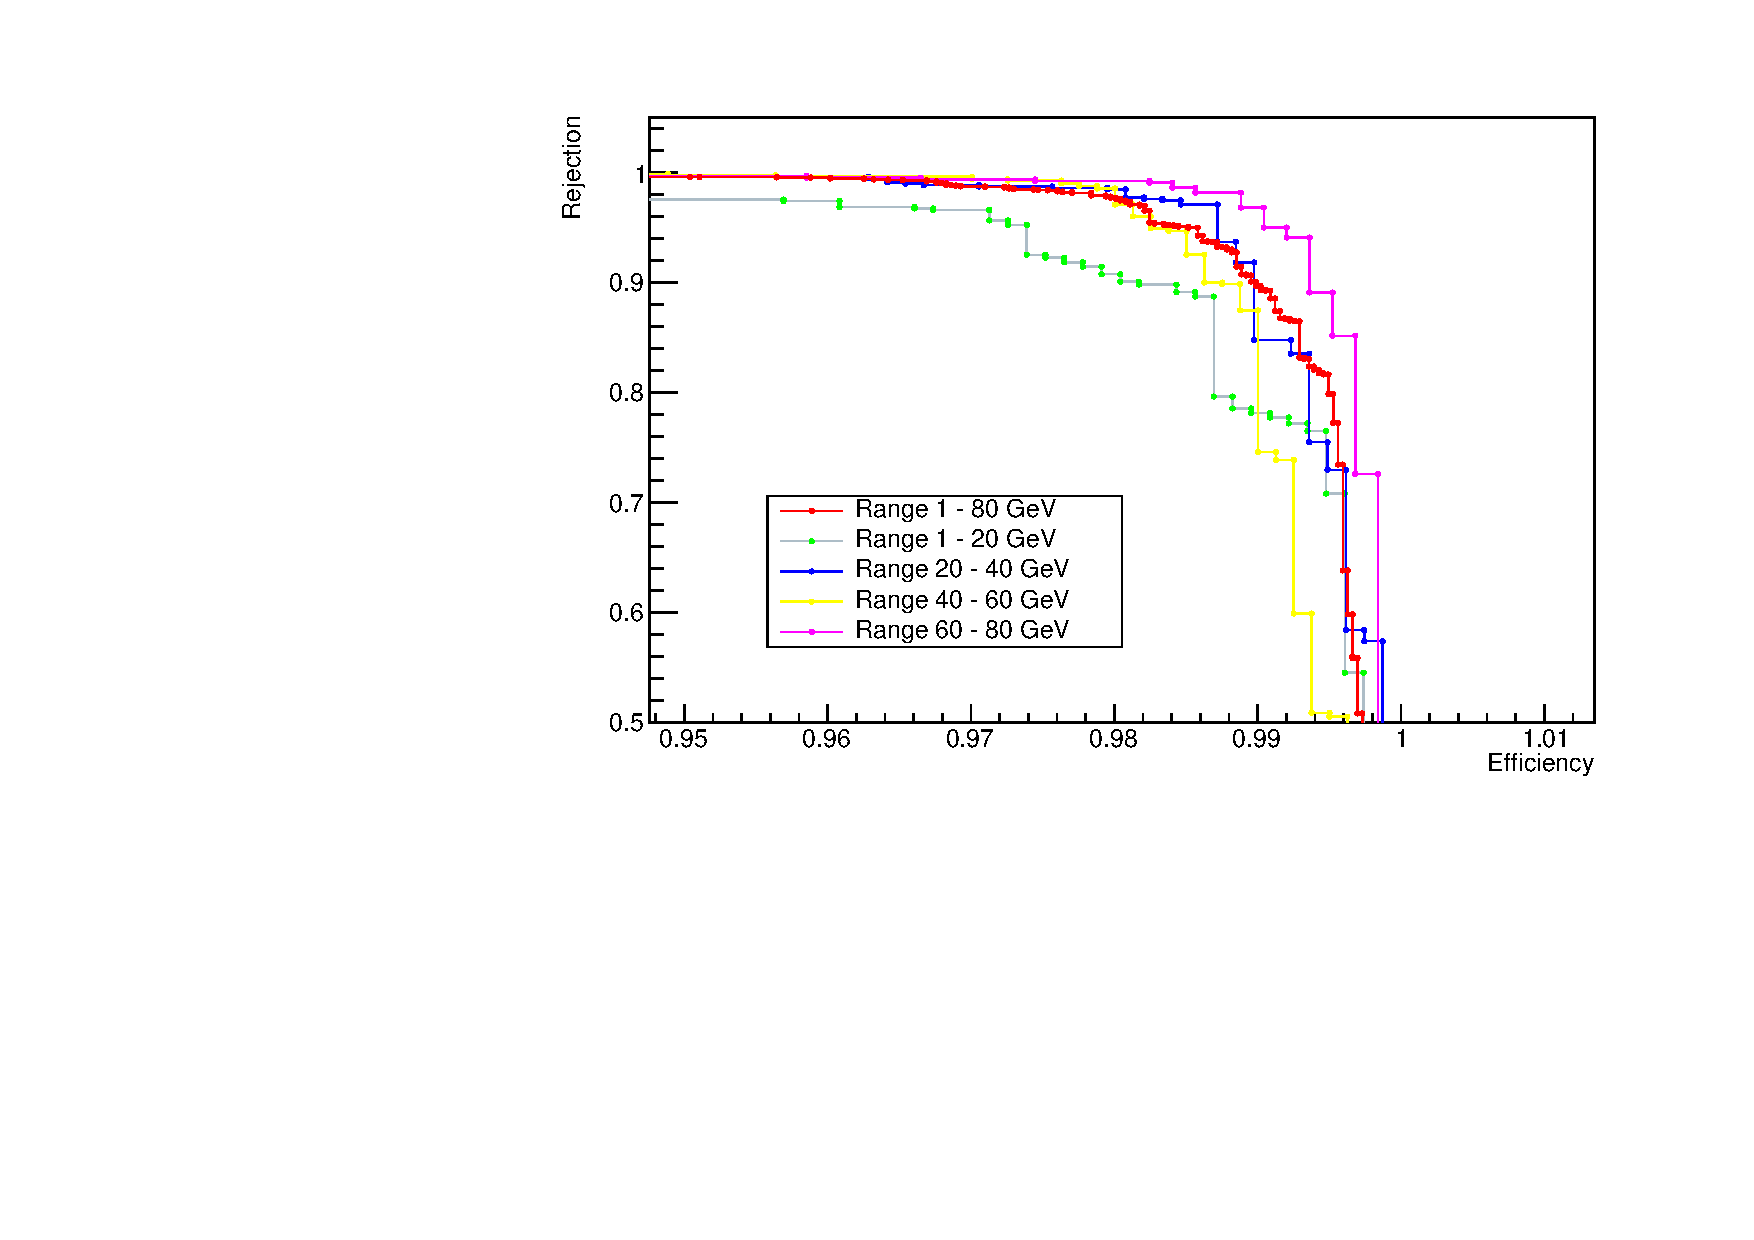
\includegraphics[width=0.85\textwidth]{IMG/Cap6/ROC_Res_sub_zoom.pdf}
	\caption{ROC curves for the selected Residual Network over subsamples of events with different energies, as described in the legend. Results for $1-80$ GeV $\pi^0/\gamma$ events simulated with the IDEA calorimeter simulation chain.}
	\label{fig:ROC_Res_sub}
\end{figure}
